\section{core\_\-oracle\_\-t Class Reference}
\label{classcore__oracle__t}\index{core\_\-oracle\_\-t@{core\_\-oracle\_\-t}}
{\tt \#include $<$zesto-oracle.h$>$}

Collaboration diagram for core\_\-oracle\_\-t:\nopagebreak
\begin{figure}[H]
\begin{center}
\leavevmode
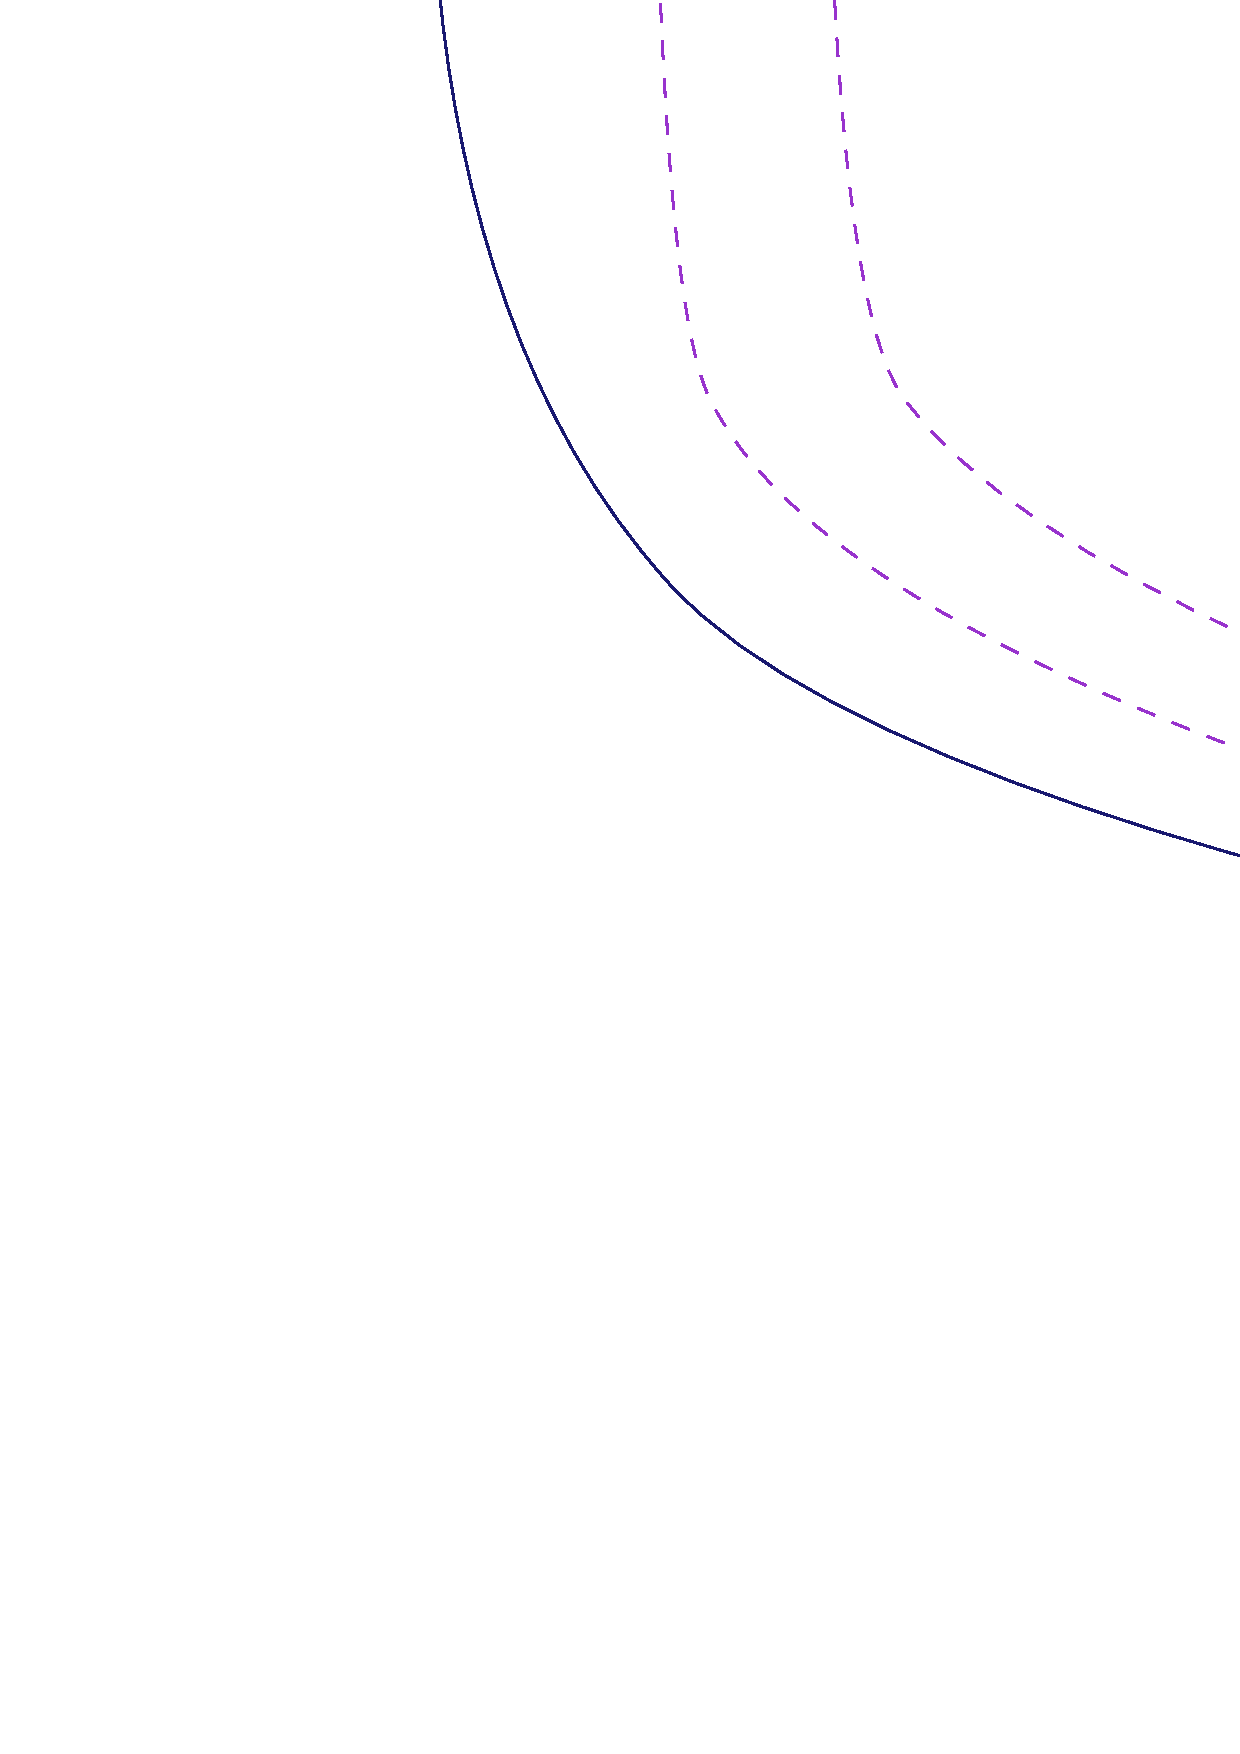
\includegraphics[width=400pt]{classcore__oracle__t__coll__graph}
\end{center}
\end{figure}
\subsection*{Classes}
\begin{CompactItemize}
\item 
struct {\bf map\_\-node\_\-t}
\item 
struct {\bf spec\_\-mem\_\-t}
\item 
struct {\bf syscall\_\-mem\_\-req\_\-t}
\end{CompactItemize}
\subsection*{Public Member Functions}
\begin{CompactItemize}
\item 
{\bf core\_\-oracle\_\-t} (struct {\bf core\_\-t} $\ast$const {\bf core})
\item 
void {\bf reg\_\-stats} (struct {\bf stat\_\-sdb\_\-t} $\ast$const sdb)
\item 
void {\bf update\_\-occupancy} (void)
\item 
struct {\bf Mop\_\-t} $\ast$ {\bf get\_\-Mop} (const int index)
\item 
int {\bf get\_\-index} (const struct {\bf Mop\_\-t} $\ast$const Mop)
\item 
int {\bf next\_\-index} (const int index)
\item 
bool {\bf spec\_\-read\_\-byte} (const {\bf md\_\-addr\_\-t} addr, {\bf byte\_\-t} $\ast$const valp)
\item 
struct {\bf spec\_\-byte\_\-t} $\ast$ {\bf spec\_\-write\_\-byte} (const {\bf md\_\-addr\_\-t} addr, const {\bf byte\_\-t} val)
\item 
struct {\bf Mop\_\-t} $\ast$ {\bf exec} (const {\bf md\_\-addr\_\-t} requested\_\-PC)
\item 
void {\bf consume} (const struct {\bf Mop\_\-t} $\ast$const Mop)
\item 
void {\bf commit\_\-uop} (struct {\bf uop\_\-t} $\ast$const uop)
\item 
void {\bf commit} (const struct {\bf Mop\_\-t} $\ast$const commit\_\-Mop)
\item 
void {\bf recover} (const struct {\bf Mop\_\-t} $\ast$const Mop)
\item 
void {\bf pipe\_\-recover} (struct {\bf Mop\_\-t} $\ast$const Mop, const {\bf md\_\-addr\_\-t} New\_\-PC)
\item 
void {\bf pipe\_\-flush} (struct {\bf Mop\_\-t} $\ast$const Mop)
\item 
void {\bf complete\_\-flush} (void)
\item 
void {\bf reset\_\-execution} (void)
\end{CompactItemize}
\subsection*{Static Public Member Functions}
\begin{CompactItemize}
\item 
static enum {\bf md\_\-fault\_\-type} {\bf syscall\_\-mem\_\-access} (int thread\_\-id, struct {\bf mem\_\-t} $\ast$mem, enum {\bf mem\_\-cmd} cmd, {\bf md\_\-addr\_\-t} addr, void $\ast$vp, int nbytes)
\end{CompactItemize}
\subsection*{Public Attributes}
\begin{CompactItemize}
\item 
bool {\bf spec\_\-mode}
\item 
bool {\bf hosed}
\item 
bool {\bf trap\_\-on}
\item 
struct {\bf map\_\-node\_\-t} $\ast$ {\bf head} [MD\_\-TOTAL\_\-REGS]
\item 
struct {\bf map\_\-node\_\-t} $\ast$ {\bf tail} [MD\_\-TOTAL\_\-REGS]
\end{CompactItemize}
\subsection*{Protected Member Functions}
\begin{CompactItemize}
\item 
void {\bf undo} (struct {\bf Mop\_\-t} $\ast$const Mop)
\item 
void {\bf install\_\-mapping} (struct {\bf uop\_\-t} $\ast$const uop)
\item 
void {\bf commit\_\-mapping} (const struct {\bf uop\_\-t} $\ast$const uop)
\item 
void {\bf undo\_\-mapping} (const struct {\bf uop\_\-t} $\ast$const uop)
\item 
struct {\bf map\_\-node\_\-t} $\ast$ {\bf get\_\-map\_\-node} (void)
\item 
void {\bf return\_\-map\_\-node} (struct {\bf map\_\-node\_\-t} $\ast$const p)
\item 
void {\bf install\_\-dependencies} (struct {\bf uop\_\-t} $\ast$const uop)
\item 
void {\bf commit\_\-dependencies} (struct {\bf uop\_\-t} $\ast$const uop)
\item 
void {\bf undo\_\-dependencies} (struct {\bf uop\_\-t} $\ast$const uop)
\item 
struct {\bf spec\_\-byte\_\-t} $\ast$ {\bf get\_\-spec\_\-mem\_\-node} (void)
\item 
void {\bf return\_\-spec\_\-mem\_\-node} (struct {\bf spec\_\-byte\_\-t} $\ast$const p)
\item 
void {\bf commit\_\-write\_\-byte} (struct {\bf spec\_\-byte\_\-t} $\ast$const p)
\item 
void {\bf squash\_\-write\_\-byte} (struct {\bf spec\_\-byte\_\-t} $\ast$const p)
\item 
void {\bf cleanup\_\-aborted\_\-mop} (struct {\bf Mop\_\-t} $\ast$const Mop)
\end{CompactItemize}
\subsection*{Static Protected Member Functions}
\begin{CompactItemize}
\item 
static void {\bf syscall\_\-callback} (void $\ast$const op)
\item 
static bool {\bf syscall\_\-translated\_\-callback} (void $\ast$const op, const {\bf seq\_\-t})
\item 
static {\bf seq\_\-t} {\bf syscall\_\-get\_\-action\_\-id} (void $\ast$const op)
\end{CompactItemize}
\subsection*{Protected Attributes}
\begin{CompactItemize}
\item 
struct {\bf Mop\_\-t} $\ast$ {\bf MopQ}
\item 
int {\bf MopQ\_\-head}
\item 
int {\bf MopQ\_\-tail}
\item 
int {\bf MopQ\_\-num}
\item 
int {\bf MopQ\_\-size}
\item 
struct {\bf Mop\_\-t} $\ast$ {\bf current\_\-Mop}
\item 
struct {\bf syscall\_\-mem\_\-req\_\-t} $\ast$ {\bf mem\_\-req\_\-free\_\-pool}
\item 
struct {\bf core\_\-t} $\ast$ {\bf core}
\item 
struct {\bf spec\_\-mem\_\-t} {\bf spec\_\-mem\_\-map}
\item 
\begin{tabbing}
xx\=xx\=xx\=xx\=xx\=xx\=xx\=xx\=xx\=\kill
struct \{\\
\>struct {\bf map\_node\_t} $\ast$ {\bf head} [MD\_TOTAL\_REGS]\\
\>struct {\bf map\_node\_t} $\ast$ {\bf tail} [MD\_TOTAL\_REGS]\\
\} {\bf dep\_map}\\

\end{tabbing}\item 
struct {\bf syscall\_\-mem\_\-req\_\-t} $\ast$ {\bf syscall\_\-mem\_\-req\_\-head}
\item 
struct {\bf syscall\_\-mem\_\-req\_\-t} $\ast$ {\bf syscall\_\-mem\_\-req\_\-tail}
\item 
int {\bf syscall\_\-mem\_\-reqs}
\item 
int {\bf syscall\_\-remaining\_\-delay}
\end{CompactItemize}
\subsection*{Static Protected Attributes}
\begin{CompactItemize}
\item 
static bool {\bf static\_\-members\_\-initialized} = false
\item 
static struct {\bf map\_\-node\_\-t} $\ast$ {\bf map\_\-free\_\-pool} = NULL
\item 
static int {\bf map\_\-free\_\-pool\_\-debt} = 0
\item 
static struct {\bf spec\_\-byte\_\-t} $\ast$ {\bf spec\_\-mem\_\-free\_\-pool} = NULL
\item 
static int {\bf spec\_\-mem\_\-pool\_\-debt} = 0
\item 
static const {\bf seq\_\-t} {\bf DUMMY\_\-SYSCALL\_\-ACTION\_\-ID} = ULL(0x2E570515CA111D)
\item 
static const unsigned {\bf DUMMY\_\-SYSCALL\_\-OP} = 0x515CA11
\end{CompactItemize}


\subsection{Detailed Description}


Definition at line 179 of file zesto-oracle.h.

\subsection{Constructor \& Destructor Documentation}
\index{core\_\-oracle\_\-t@{core\_\-oracle\_\-t}!core\_\-oracle\_\-t@{core\_\-oracle\_\-t}}
\index{core\_\-oracle\_\-t@{core\_\-oracle\_\-t}!core_oracle_t@{core\_\-oracle\_\-t}}
\subsubsection[{core\_\-oracle\_\-t}]{\setlength{\rightskip}{0pt plus 5cm}core\_\-oracle\_\-t::core\_\-oracle\_\-t (struct {\bf core\_\-t} $\ast$const  {\em core})}\label{classcore__oracle__t_ee5b386437040a0500ffbc2a677a52d3}




Definition at line 178 of file zesto-oracle.cpp.

References core\_\-knobs\_\-t::alloc, core\_\-knobs\_\-t::byteQ\_\-size, core\_\-knobs\_\-t::commit, core, core\_\-knobs\_\-t::decode, dep\_\-map, core\_\-knobs\_\-t::depth, fatal(), core\_\-knobs\_\-t::fetch, core\_\-knobs\_\-t::IQ\_\-size, core\_\-t::knobs, knobs, MopQ, MopQ\_\-size, core\_\-knobs\_\-t::ROB\_\-size, spec\_\-mem\_\-map, core\_\-knobs\_\-t::uopQ\_\-size, and core\_\-knobs\_\-t::width.

\subsection{Member Function Documentation}
\index{core\_\-oracle\_\-t@{core\_\-oracle\_\-t}!cleanup\_\-aborted\_\-mop@{cleanup\_\-aborted\_\-mop}}
\index{cleanup\_\-aborted\_\-mop@{cleanup\_\-aborted\_\-mop}!core_oracle_t@{core\_\-oracle\_\-t}}
\subsubsection[{cleanup\_\-aborted\_\-mop}]{\setlength{\rightskip}{0pt plus 5cm}void core\_\-oracle\_\-t::cleanup\_\-aborted\_\-mop (struct {\bf Mop\_\-t} $\ast$const  {\em Mop})\hspace{0.3cm}{\tt  [protected]}}\label{classcore__oracle__t_ba04cbb4ec9ba6ffb03455a2f5c5da32}




Definition at line 2203 of file zesto-oracle.cpp.

References uop\_\-t::decode, Mop\_\-t::decode, Mop\_\-t::flow\_\-length, uop\_\-t::is\_\-imm, uop\_\-t::oracle, uop\_\-t::spec\_\-mem, and Mop\_\-t::uop.\index{core\_\-oracle\_\-t@{core\_\-oracle\_\-t}!commit@{commit}}
\index{commit@{commit}!core_oracle_t@{core\_\-oracle\_\-t}}
\subsubsection[{commit}]{\setlength{\rightskip}{0pt plus 5cm}void core\_\-oracle\_\-t::commit (const struct {\bf Mop\_\-t} $\ast$const  {\em commit\_\-Mop})}\label{classcore__oracle__t_5656906c0caee72b39f9d3760341de99}




Definition at line 1562 of file zesto-oracle.cpp.

References fatal(), modinc(), MopQ, MopQ\_\-head, MopQ\_\-num, MopQ\_\-size, Mop\_\-t::oracle, Mop\_\-t::spec\_\-mode, and Mop\_\-t::valid.

Referenced by core\_\-commit\_\-STM\_\-t::step(), and core\_\-commit\_\-DPM\_\-t::step().

Here is the caller graph for this function:\nopagebreak
\begin{figure}[H]
\begin{center}
\leavevmode
\includegraphics[width=163pt]{classcore__oracle__t_5656906c0caee72b39f9d3760341de99_icgraph}
\end{center}
\end{figure}
\index{core\_\-oracle\_\-t@{core\_\-oracle\_\-t}!commit\_\-dependencies@{commit\_\-dependencies}}
\index{commit\_\-dependencies@{commit\_\-dependencies}!core_oracle_t@{core\_\-oracle\_\-t}}
\subsubsection[{commit\_\-dependencies}]{\setlength{\rightskip}{0pt plus 5cm}void core\_\-oracle\_\-t::commit\_\-dependencies (struct {\bf uop\_\-t} $\ast$const  {\em uop})\hspace{0.3cm}{\tt  [protected]}}\label{classcore__oracle__t_999bfe83c41ad19d351d0cfc5cc1b16a}




Definition at line 1848 of file zesto-oracle.cpp.

References core, uop\_\-t::idep\_\-uop, odep\_\-t::next, uop\_\-t::odep\_\-uop, odep\_\-t::op\_\-num, uop\_\-t::oracle, core\_\-t::return\_\-odep\_\-link(), and odep\_\-t::uop.

Referenced by commit\_\-uop().

Here is the caller graph for this function:\nopagebreak
\begin{figure}[H]
\begin{center}
\leavevmode
\includegraphics[width=280pt]{classcore__oracle__t_999bfe83c41ad19d351d0cfc5cc1b16a_icgraph}
\end{center}
\end{figure}
\index{core\_\-oracle\_\-t@{core\_\-oracle\_\-t}!commit\_\-mapping@{commit\_\-mapping}}
\index{commit\_\-mapping@{commit\_\-mapping}!core_oracle_t@{core\_\-oracle\_\-t}}
\subsubsection[{commit\_\-mapping}]{\setlength{\rightskip}{0pt plus 5cm}void core\_\-oracle\_\-t::commit\_\-mapping (const struct {\bf uop\_\-t} $\ast$const  {\em uop})\hspace{0.3cm}{\tt  [protected]}}\label{classcore__oracle__t_9c6462ead2fb5d7d4134ff11fc918029}




Definition at line 1798 of file zesto-oracle.cpp.

References DCREG, uop\_\-t::decode, dep\_\-map, DGPR, DNA, MD\_\-REG\_\-AFLAGS, MD\_\-REG\_\-ZERO, core\_\-oracle\_\-t::core\_\-oracle\_\-t::map\_\-node\_\-t::next, uop\_\-t::odep\_\-name, uop\_\-t::oflags, core\_\-oracle\_\-t::core\_\-oracle\_\-t::map\_\-node\_\-t::prev, return\_\-map\_\-node(), and core\_\-oracle\_\-t::core\_\-oracle\_\-t::map\_\-node\_\-t::uop.

Referenced by commit\_\-uop().

Here is the caller graph for this function:\nopagebreak
\begin{figure}[H]
\begin{center}
\leavevmode
\includegraphics[width=269pt]{classcore__oracle__t_9c6462ead2fb5d7d4134ff11fc918029_icgraph}
\end{center}
\end{figure}
\index{core\_\-oracle\_\-t@{core\_\-oracle\_\-t}!commit\_\-uop@{commit\_\-uop}}
\index{commit\_\-uop@{commit\_\-uop}!core_oracle_t@{core\_\-oracle\_\-t}}
\subsubsection[{commit\_\-uop}]{\setlength{\rightskip}{0pt plus 5cm}void core\_\-oracle\_\-t::commit\_\-uop (struct {\bf uop\_\-t} $\ast$const  {\em uop})}\label{classcore__oracle__t_ba02df09c524181a44404676f33669a5}




Definition at line 1527 of file zesto-oracle.cpp.

References commit\_\-dependencies(), commit\_\-mapping(), core, uop\_\-t::exec, uop\_\-t::idep\_\-uop, odep\_\-t::next, uop\_\-t::odep\_\-uop, odep\_\-t::op\_\-num, core\_\-t::return\_\-odep\_\-link(), odep\_\-t::uop, and zesto\_\-assert.

Referenced by core\_\-commit\_\-STM\_\-t::step(), and core\_\-commit\_\-DPM\_\-t::step().

Here is the caller graph for this function:\nopagebreak
\begin{figure}[H]
\begin{center}
\leavevmode
\includegraphics[width=173pt]{classcore__oracle__t_ba02df09c524181a44404676f33669a5_icgraph}
\end{center}
\end{figure}
\index{core\_\-oracle\_\-t@{core\_\-oracle\_\-t}!commit\_\-write\_\-byte@{commit\_\-write\_\-byte}}
\index{commit\_\-write\_\-byte@{commit\_\-write\_\-byte}!core_oracle_t@{core\_\-oracle\_\-t}}
\subsubsection[{commit\_\-write\_\-byte}]{\setlength{\rightskip}{0pt plus 5cm}void core\_\-oracle\_\-t::commit\_\-write\_\-byte (struct {\bf spec\_\-byte\_\-t} $\ast$const  {\em p})\hspace{0.3cm}{\tt  [protected]}}\label{classcore__oracle__t_084f475b2682976f22fbad98943ac04f}




Definition at line 1870 of file zesto-oracle.cpp.

References spec\_\-byte\_\-t::addr, core\_\-oracle\_\-t::core\_\-oracle\_\-t::spec\_\-mem\_\-t::hash, core\_\-oracle\_\-t::core\_\-oracle\_\-t::spec\_\-mem\_\-t::head, MEM\_\-HASH\_\-MASK, spec\_\-byte\_\-t::next, spec\_\-byte\_\-t::prev, return\_\-spec\_\-mem\_\-node(), spec\_\-mem\_\-map, and core\_\-oracle\_\-t::core\_\-oracle\_\-t::spec\_\-mem\_\-t::tail.\index{core\_\-oracle\_\-t@{core\_\-oracle\_\-t}!complete\_\-flush@{complete\_\-flush}}
\index{complete\_\-flush@{complete\_\-flush}!core_oracle_t@{core\_\-oracle\_\-t}}
\subsubsection[{complete\_\-flush}]{\setlength{\rightskip}{0pt plus 5cm}void core\_\-oracle\_\-t::complete\_\-flush (void)}\label{classcore__oracle__t_9f125e90b225555a2632277161f3b27c}




Definition at line 1747 of file zesto-oracle.cpp.

References core\_\-fetch\_\-t::bpred, Mop\_\-t::bpred\_\-update, core, current\_\-Mop, core\_\-t::current\_\-thread, core\_\-t::fetch, Mop\_\-t::fetch, bpred\_\-t::flush(), moddec(), MopQ, MopQ\_\-head, MopQ\_\-num, MopQ\_\-size, MopQ\_\-tail, Mop\_\-t::PC, thread\_\-t::regs, regs\_\-t::regs\_\-NPC, regs\_\-t::regs\_\-PC, bpred\_\-t::return\_\-state\_\-cache(), spec\_\-mode, undo(), and Mop\_\-t::valid.

Referenced by emergency\_\-recovery(), reset\_\-execution(), core\_\-commit\_\-STM\_\-t::step(), and core\_\-commit\_\-DPM\_\-t::step().

Here is the caller graph for this function:\nopagebreak
\begin{figure}[H]
\begin{center}
\leavevmode
\includegraphics[width=420pt]{classcore__oracle__t_9f125e90b225555a2632277161f3b27c_icgraph}
\end{center}
\end{figure}
\index{core\_\-oracle\_\-t@{core\_\-oracle\_\-t}!consume@{consume}}
\index{consume@{consume}!core_oracle_t@{core\_\-oracle\_\-t}}
\subsubsection[{consume}]{\setlength{\rightskip}{0pt plus 5cm}void core\_\-oracle\_\-t::consume (const struct {\bf Mop\_\-t} $\ast$const  {\em Mop})}\label{classcore__oracle__t_527c3d85c2b86a3fed4c223b529dd33f}




Definition at line 1519 of file zesto-oracle.cpp.

References current\_\-Mop.

Referenced by core\_\-fetch\_\-STM\_\-t::step(), and core\_\-fetch\_\-DPM\_\-t::step().

Here is the caller graph for this function:\nopagebreak
\begin{figure}[H]
\begin{center}
\leavevmode
\includegraphics[width=161pt]{classcore__oracle__t_527c3d85c2b86a3fed4c223b529dd33f_icgraph}
\end{center}
\end{figure}
\index{core\_\-oracle\_\-t@{core\_\-oracle\_\-t}!exec@{exec}}
\index{exec@{exec}!core_oracle_t@{core\_\-oracle\_\-t}}
\subsubsection[{exec}]{\setlength{\rightskip}{0pt plus 5cm}struct {\bf Mop\_\-t} $\ast$ core\_\-oracle\_\-t::exec (const {\bf md\_\-addr\_\-t} {\em requested\_\-PC})\hspace{0.3cm}{\tt  [read]}}\label{classcore__oracle__t_1ac2b1204cef575e22d1d03c3ce4cff9}




Definition at line 669 of file zesto-oracle.cpp.

References core\_\-fetch\_\-t::bogus, uop\_\-t::BOM, md\_\-inst\_\-t::code, Mop\_\-t::core, core, current\_\-Mop, core\_\-t::current\_\-thread, core\_\-knobs\_\-t::decode, uop\_\-t::decode, Mop\_\-t::decode, DNA, uop\_\-t::EOM, F\_\-COND, F\_\-CTRL, F\_\-FENCE, F\_\-LOAD, F\_\-MEM, F\_\-STORE, F\_\-TRAP, F\_\-UCODE, fatal(), uop\_\-t::fault, Mop\_\-t::fetch, core\_\-t::fetch, Mop\_\-t::first\_\-rep, uop\_\-t::flow\_\-index, Mop\_\-t::flow\_\-length, FPSTACK\_\-IMPL, Mop\_\-t::fpstack\_\-op, fpstk\_\-nop, uop\_\-t::FU\_\-class, uop\_\-t::fusion\_\-head, core\_\-knobs\_\-t::fusion\_\-mode, uop\_\-t::fusion\_\-next, uop\_\-t::fusion\_\-size, FUSION\_\-TYPE, core\_\-t::get\_\-uop\_\-array(), core\_\-t::global\_\-seq, uop\_\-t::has\_\-imm, core\_\-t::id, uop\_\-t::idep\_\-name, md\_\-inst\_\-t::imm, uop\_\-t::in\_\-fusion, Mop\_\-t::inst, install\_\-dependencies(), install\_\-mapping(), uop\_\-t::is\_\-ctrl, Mop\_\-t::is\_\-ctrl, uop\_\-t::is\_\-fusion\_\-head, uop\_\-t::is\_\-imm, uop\_\-t::is\_\-load, uop\_\-t::is\_\-nop, uop\_\-t::is\_\-sta, uop\_\-t::is\_\-std, Mop\_\-t::is\_\-trap, core\_\-t::knobs, knobs, Mop\_\-t::last\_\-uop\_\-index, mem\_\-ops::ld\_\-dequeued, mem\_\-ops::ld\_\-size, md\_\-inst\_\-t::len, uncore\_\-t::log\_\-trace, md\_\-fault\_\-none, MD\_\-FETCH\_\-INST, MD\_\-FETCH\_\-NEXT\_\-PC, md\_\-get\_\-flow(), MD\_\-INC\_\-FLOW, MD\_\-INST\_\-SIZE, MD\_\-MAX\_\-FLOWLEN, MD\_\-NOP\_\-INST, MD\_\-OP\_\-FLAGS, MD\_\-OP\_\-FUCLASS, MD\_\-SET\_\-OPCODE\_\-DURING\_\-FETCH, MD\_\-SET\_\-UOPCODE, MD\_\-STA\_\-OP\_\-INDEX, MD\_\-TOTAL\_\-REGS, md\_\-uop\_\-immb(), md\_\-uop\_\-opc(), md\_\-uop\_\-reg(), thread\_\-t::mem, md\_\-inst\_\-t::mem\_\-ops, mem\_\-ops::mem\_\-paddr\_\-ld, mem\_\-ops::mem\_\-paddr\_\-str, uop\_\-t::mem\_\-size, mem\_\-ops::mem\_\-vaddr\_\-ld, mem\_\-ops::mem\_\-vaddr\_\-str, mem\_\-ops::memops, md\_\-inst\_\-t::mode, MODE\_\-ADDR32, modinc(), uop\_\-t::Mop, uop\_\-t::Mop\_\-seq, MopQ, MopQ\_\-num, MopQ\_\-size, MopQ\_\-tail, Mop\_\-t::NextPC, Mop\_\-t::num\_\-branches, Mop\_\-t::num\_\-eff\_\-uops, thread\_\-t::num\_\-insn, Mop\_\-t::num\_\-loads, Mop\_\-t::num\_\-refs, Mop\_\-t::num\_\-uops, uop\_\-t::odep\_\-name, uop\_\-t::op, Mop\_\-t::op, OP\_\-NA, uop\_\-t::opflags, Mop\_\-t::opflags, uop\_\-t::oracle, Mop\_\-t::oracle, core\_\-t::core\_\-t::core\_\-stat\_\-t::oracle\_\-bogus\_\-cycles, core\_\-t::core\_\-t::core\_\-stat\_\-t::oracle\_\-num\_\-branches, core\_\-t::core\_\-t::core\_\-stat\_\-t::oracle\_\-num\_\-loads, core\_\-t::core\_\-t::core\_\-stat\_\-t::oracle\_\-num\_\-refs, core\_\-t::core\_\-t::core\_\-stat\_\-t::oracle\_\-total\_\-branches, core\_\-t::core\_\-t::core\_\-stat\_\-t::oracle\_\-total\_\-eff\_\-uops, core\_\-t::core\_\-t::core\_\-stat\_\-t::oracle\_\-total\_\-insn, core\_\-t::core\_\-t::core\_\-stat\_\-t::oracle\_\-total\_\-loads, core\_\-t::core\_\-t::core\_\-stat\_\-t::oracle\_\-total\_\-refs, core\_\-t::core\_\-t::core\_\-stat\_\-t::oracle\_\-total\_\-uops, md\_\-inst\_\-t::paddr, panic(), Mop\_\-t::PC, uop\_\-t::phys\_\-addr, Mop\_\-t::pred\_\-NPC, md\_\-inst\_\-t::qemu\_\-len, R, uop\_\-t::raw\_\-op, thread\_\-t::regs, regs\_\-t::regs\_\-NPC, regs\_\-t::regs\_\-PC, md\_\-inst\_\-t::rep, REP\_\-REP, REP\_\-REPNZ, REP\_\-REPZ, Mop\_\-t::rep\_\-seq, thread\_\-t::rep\_\-sequence, core\_\-t::return\_\-uop\_\-array(), RM, Mop\_\-t::seq, Mop\_\-t::spec\_\-mode, spec\_\-mode, thread\_\-t::stat, Mop\_\-t::stat, core\_\-t::stat, mem\_\-ops::str\_\-dequeued, mem\_\-ops::str\_\-size, Mop\_\-t::targetPC, TICK\_\-T\_\-MAX, Mop\_\-t::timing, uop\_\-t::timing, UHASIMM, core\_\-t::uncore, Mop\_\-t::uop, uop\_\-t::uop\_\-seq, UOP\_\-SEQ\_\-SHIFT, UP, md\_\-inst\_\-t::vaddr, Mop\_\-t::valid, uop\_\-t::virt\_\-addr, warn(), Mop\_\-t::when\_\-commit\_\-finished, Mop\_\-t::when\_\-commit\_\-started, uop\_\-t::when\_\-completed, Mop\_\-t::when\_\-decode\_\-finished, Mop\_\-t::when\_\-decode\_\-started, uop\_\-t::when\_\-exec, Mop\_\-t::when\_\-fetch\_\-started, Mop\_\-t::when\_\-fetched, uop\_\-t::when\_\-issued, Mop\_\-t::when\_\-MS\_\-started, uop\_\-t::when\_\-ready, XE\_\-ONE, XR\_\-CX, XR\_\-ECX, core\_\-t::zero\_\-Mop(), Mop\_\-t::zero\_\-rep, and ZESTO\_\-STAT.

Referenced by core\_\-fetch\_\-STM\_\-t::step(), and core\_\-fetch\_\-DPM\_\-t::step().

Here is the caller graph for this function:\nopagebreak
\begin{figure}[H]
\begin{center}
\leavevmode
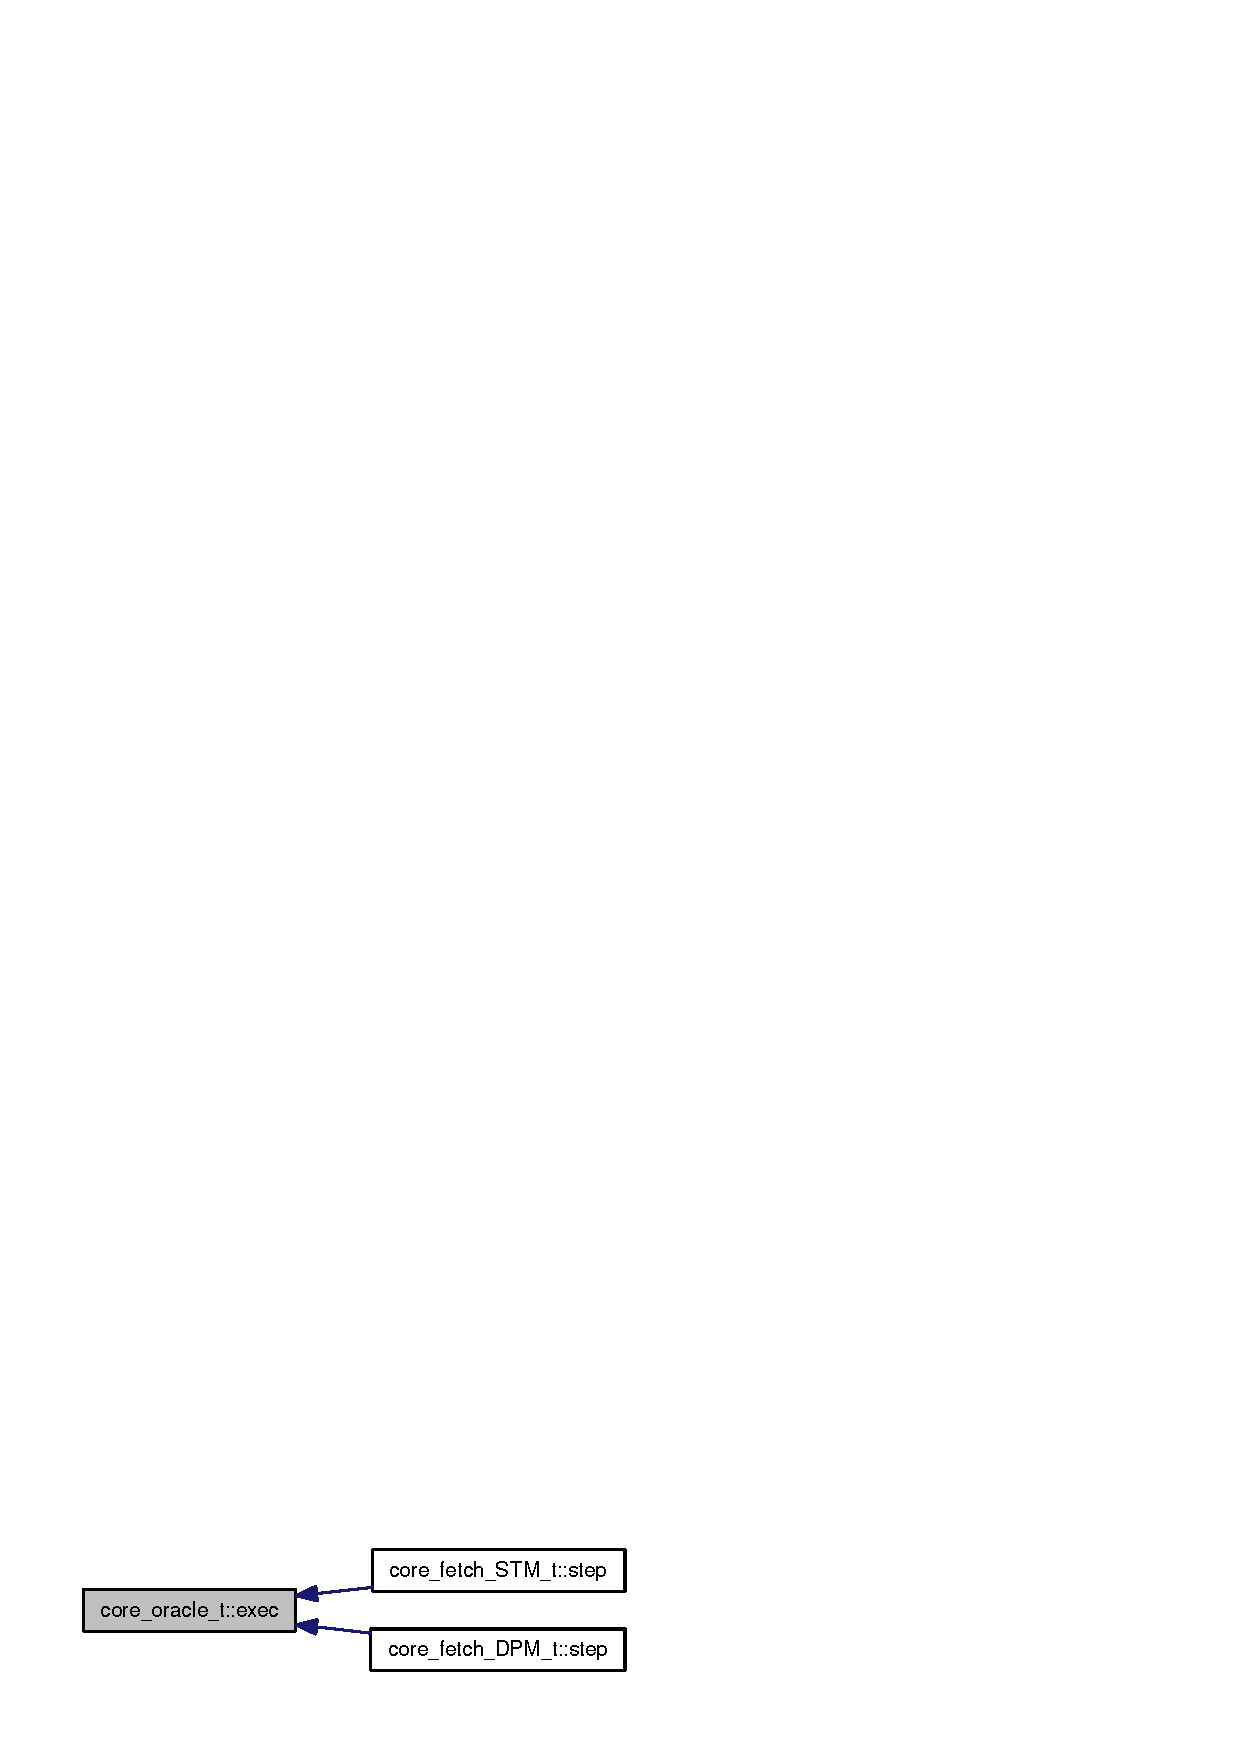
\includegraphics[width=152pt]{classcore__oracle__t_1ac2b1204cef575e22d1d03c3ce4cff9_icgraph}
\end{center}
\end{figure}
\index{core\_\-oracle\_\-t@{core\_\-oracle\_\-t}!get\_\-index@{get\_\-index}}
\index{get\_\-index@{get\_\-index}!core_oracle_t@{core\_\-oracle\_\-t}}
\subsubsection[{get\_\-index}]{\setlength{\rightskip}{0pt plus 5cm}int core\_\-oracle\_\-t::get\_\-index (const struct {\bf Mop\_\-t} $\ast$const  {\em Mop})}\label{classcore__oracle__t_2c1b1e382fd5cd3a13a52560adf9ce7b}




Definition at line 340 of file zesto-oracle.cpp.

References MopQ.

Referenced by core\_\-fetch\_\-STM\_\-t::step(), and core\_\-fetch\_\-DPM\_\-t::step().

Here is the caller graph for this function:\nopagebreak
\begin{figure}[H]
\begin{center}
\leavevmode
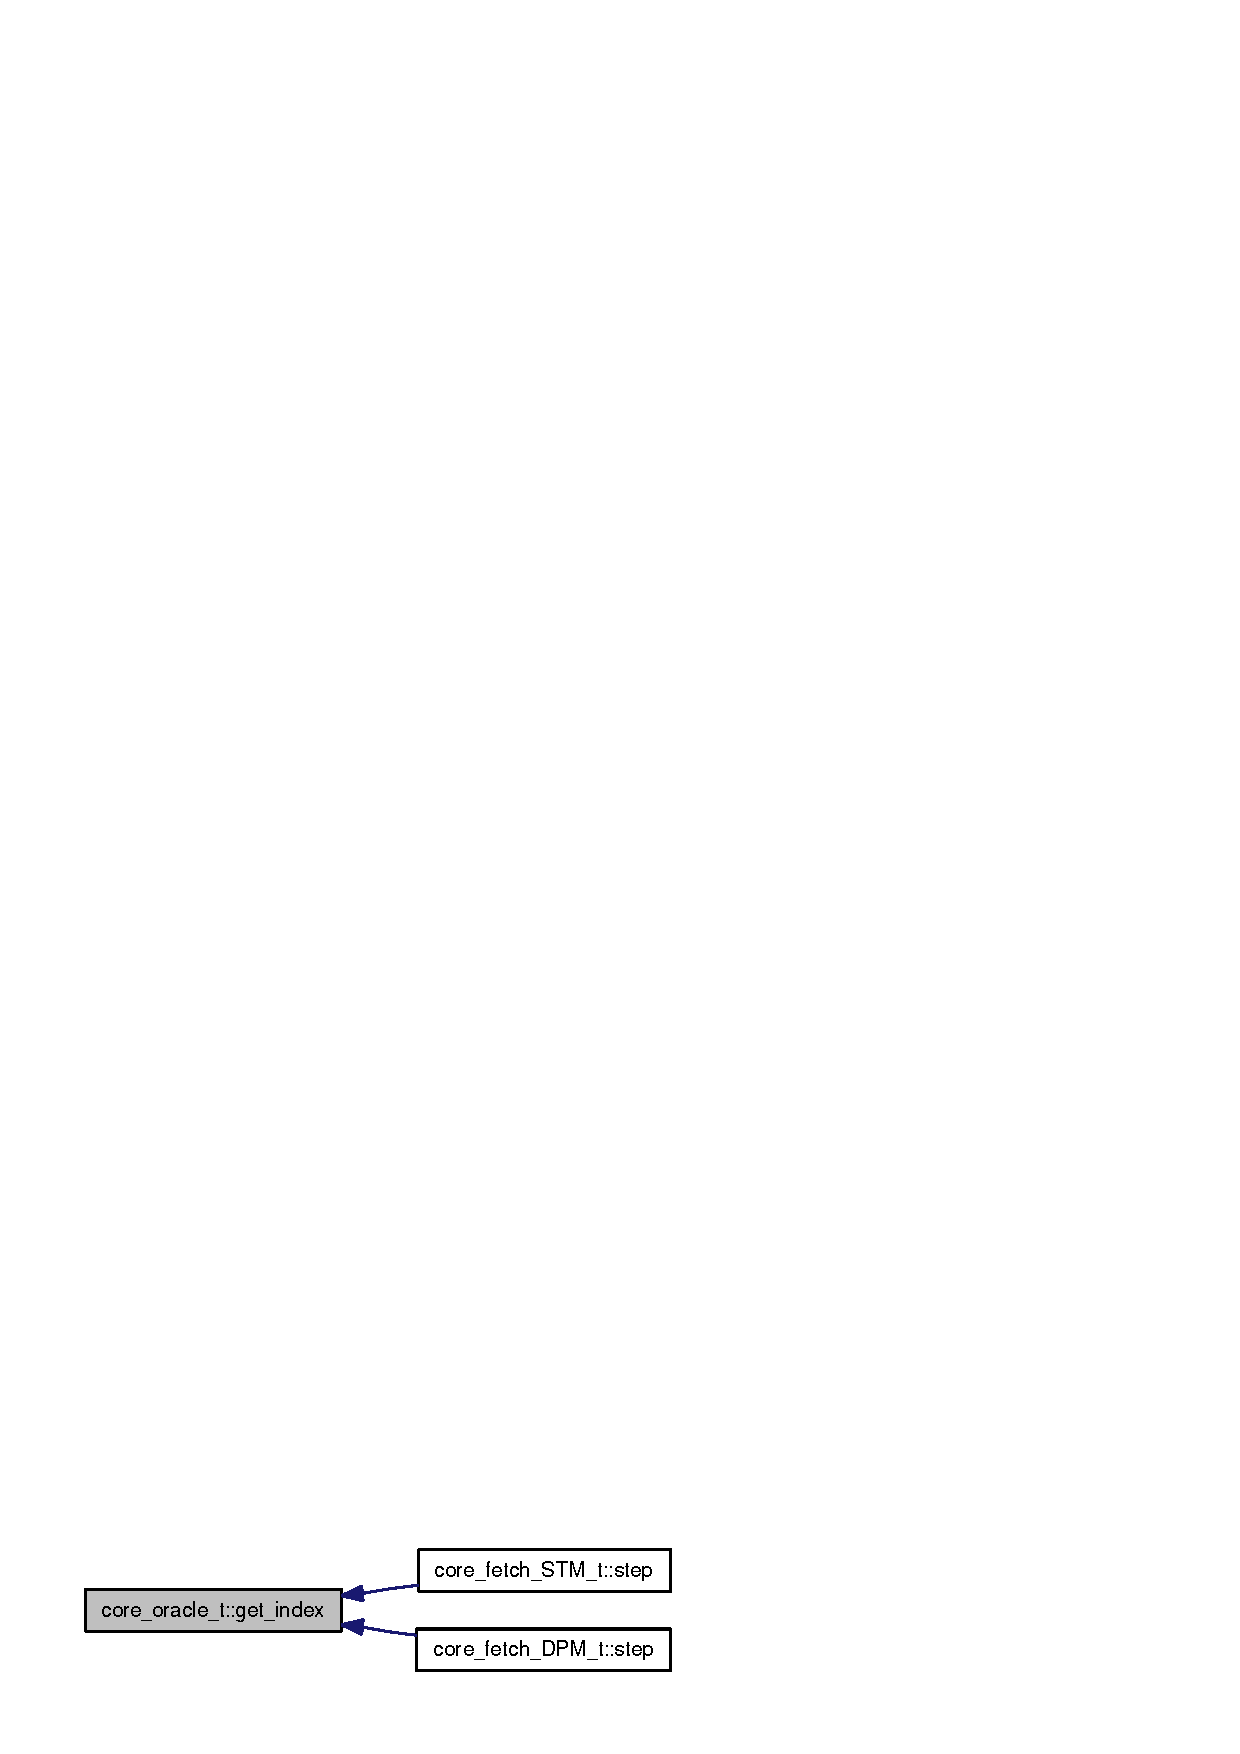
\includegraphics[width=163pt]{classcore__oracle__t_2c1b1e382fd5cd3a13a52560adf9ce7b_icgraph}
\end{center}
\end{figure}
\index{core\_\-oracle\_\-t@{core\_\-oracle\_\-t}!get\_\-map\_\-node@{get\_\-map\_\-node}}
\index{get\_\-map\_\-node@{get\_\-map\_\-node}!core_oracle_t@{core\_\-oracle\_\-t}}
\subsubsection[{get\_\-map\_\-node}]{\setlength{\rightskip}{0pt plus 5cm}struct {\bf core\_\-oracle\_\-t::map\_\-node\_\-t} $\ast$ core\_\-oracle\_\-t::get\_\-map\_\-node (void)\hspace{0.3cm}{\tt  [read, protected]}}\label{classcore__oracle__t_1d625a959241c89446eb56ea68c374cc}




Definition at line 2014 of file zesto-oracle.cpp.

References fatal(), map\_\-free\_\-pool, map\_\-free\_\-pool\_\-debt, and core\_\-oracle\_\-t::core\_\-oracle\_\-t::map\_\-node\_\-t::next.

Referenced by install\_\-mapping().

Here is the caller graph for this function:\nopagebreak
\begin{figure}[H]
\begin{center}
\leavevmode
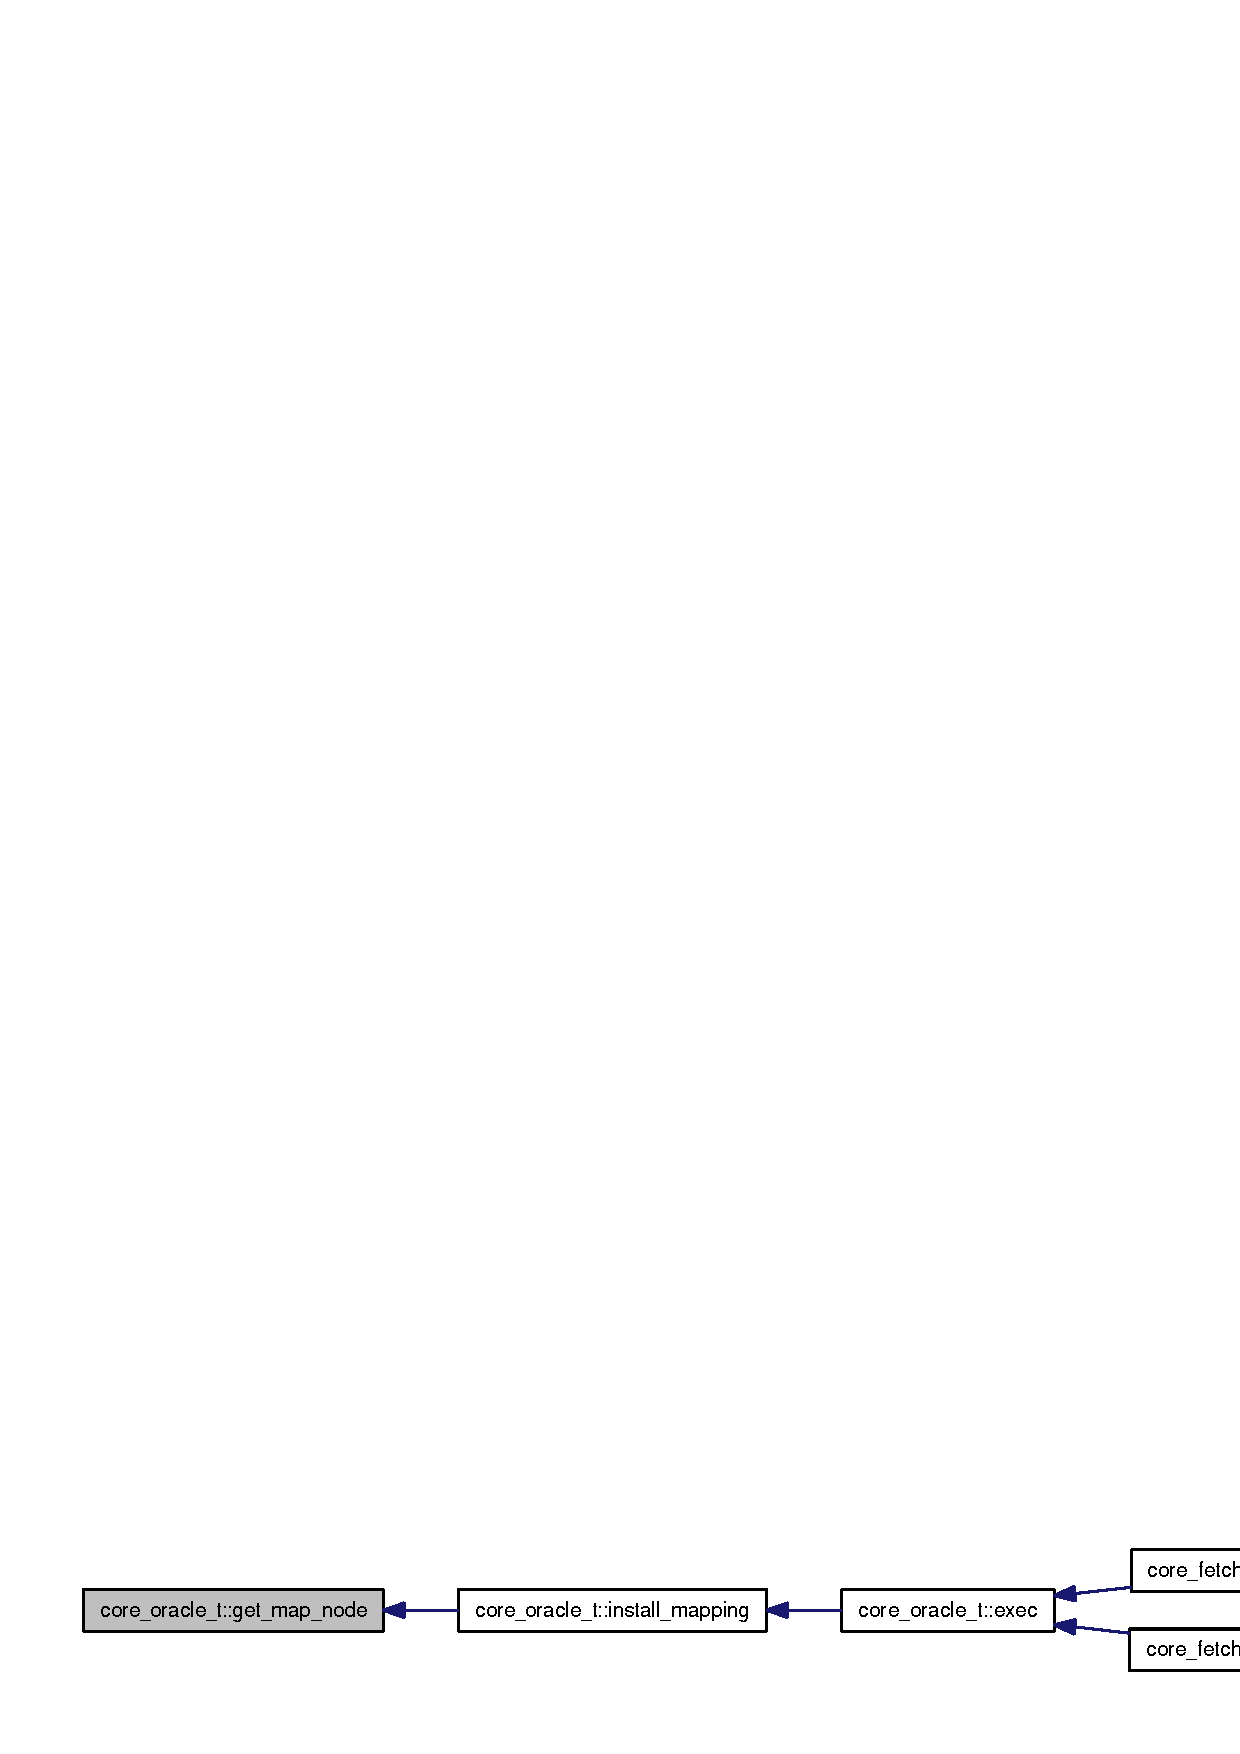
\includegraphics[width=334pt]{classcore__oracle__t_1d625a959241c89446eb56ea68c374cc_icgraph}
\end{center}
\end{figure}
\index{core\_\-oracle\_\-t@{core\_\-oracle\_\-t}!get\_\-Mop@{get\_\-Mop}}
\index{get\_\-Mop@{get\_\-Mop}!core_oracle_t@{core\_\-oracle\_\-t}}
\subsubsection[{get\_\-Mop}]{\setlength{\rightskip}{0pt plus 5cm}struct {\bf Mop\_\-t} $\ast$ core\_\-oracle\_\-t::get\_\-Mop (const int {\em index})\hspace{0.3cm}{\tt  [read]}}\label{classcore__oracle__t_476405605981d10733d94063d4441dfe}




Definition at line 335 of file zesto-oracle.cpp.

References MopQ.

Referenced by core\_\-fetch\_\-STM\_\-t::Mop\_\-consume(), core\_\-fetch\_\-STM\_\-t::Mop\_\-peek(), and core\_\-fetch\_\-DPM\_\-t::step().

Here is the caller graph for this function:\nopagebreak
\begin{figure}[H]
\begin{center}
\leavevmode
\includegraphics[width=182pt]{classcore__oracle__t_476405605981d10733d94063d4441dfe_icgraph}
\end{center}
\end{figure}
\index{core\_\-oracle\_\-t@{core\_\-oracle\_\-t}!get\_\-spec\_\-mem\_\-node@{get\_\-spec\_\-mem\_\-node}}
\index{get\_\-spec\_\-mem\_\-node@{get\_\-spec\_\-mem\_\-node}!core_oracle_t@{core\_\-oracle\_\-t}}
\subsubsection[{get\_\-spec\_\-mem\_\-node}]{\setlength{\rightskip}{0pt plus 5cm}struct {\bf spec\_\-byte\_\-t} $\ast$ core\_\-oracle\_\-t::get\_\-spec\_\-mem\_\-node (void)\hspace{0.3cm}{\tt  [read, protected]}}\label{classcore__oracle__t_b4d62e47b0d6399f7fc7738eb0864f17}




Definition at line 2150 of file zesto-oracle.cpp.

References fatal(), spec\_\-byte\_\-t::next, and spec\_\-mem\_\-free\_\-pool.

Referenced by spec\_\-write\_\-byte().

Here is the caller graph for this function:\nopagebreak
\begin{figure}[H]
\begin{center}
\leavevmode
\includegraphics[width=203pt]{classcore__oracle__t_b4d62e47b0d6399f7fc7738eb0864f17_icgraph}
\end{center}
\end{figure}
\index{core\_\-oracle\_\-t@{core\_\-oracle\_\-t}!install\_\-dependencies@{install\_\-dependencies}}
\index{install\_\-dependencies@{install\_\-dependencies}!core_oracle_t@{core\_\-oracle\_\-t}}
\subsubsection[{install\_\-dependencies}]{\setlength{\rightskip}{0pt plus 5cm}void core\_\-oracle\_\-t::install\_\-dependencies (struct {\bf uop\_\-t} $\ast$const  {\em uop})\hspace{0.3cm}{\tt  [protected]}}\label{classcore__oracle__t_deeae95a29f95000a81b20fb895a2e64}




Definition at line 2049 of file zesto-oracle.cpp.

References odep\_\-t::aflags, core, DCREG, uop\_\-t::decode, dep\_\-map, DNA, core\_\-t::get\_\-odep\_\-link(), uop\_\-t::idep\_\-name, uop\_\-t::idep\_\-uop, uop\_\-t::iflags, MAX\_\-IDEPS, MD\_\-REG\_\-AFLAGS, MD\_\-REG\_\-ZERO, uop\_\-t::Mop, odep\_\-t::next, uop\_\-t::odep\_\-uop, odep\_\-t::op\_\-num, Mop\_\-t::oracle, uop\_\-t::oracle, Mop\_\-t::seq, and odep\_\-t::uop.

Referenced by exec().

Here is the caller graph for this function:\nopagebreak
\begin{figure}[H]
\begin{center}
\leavevmode
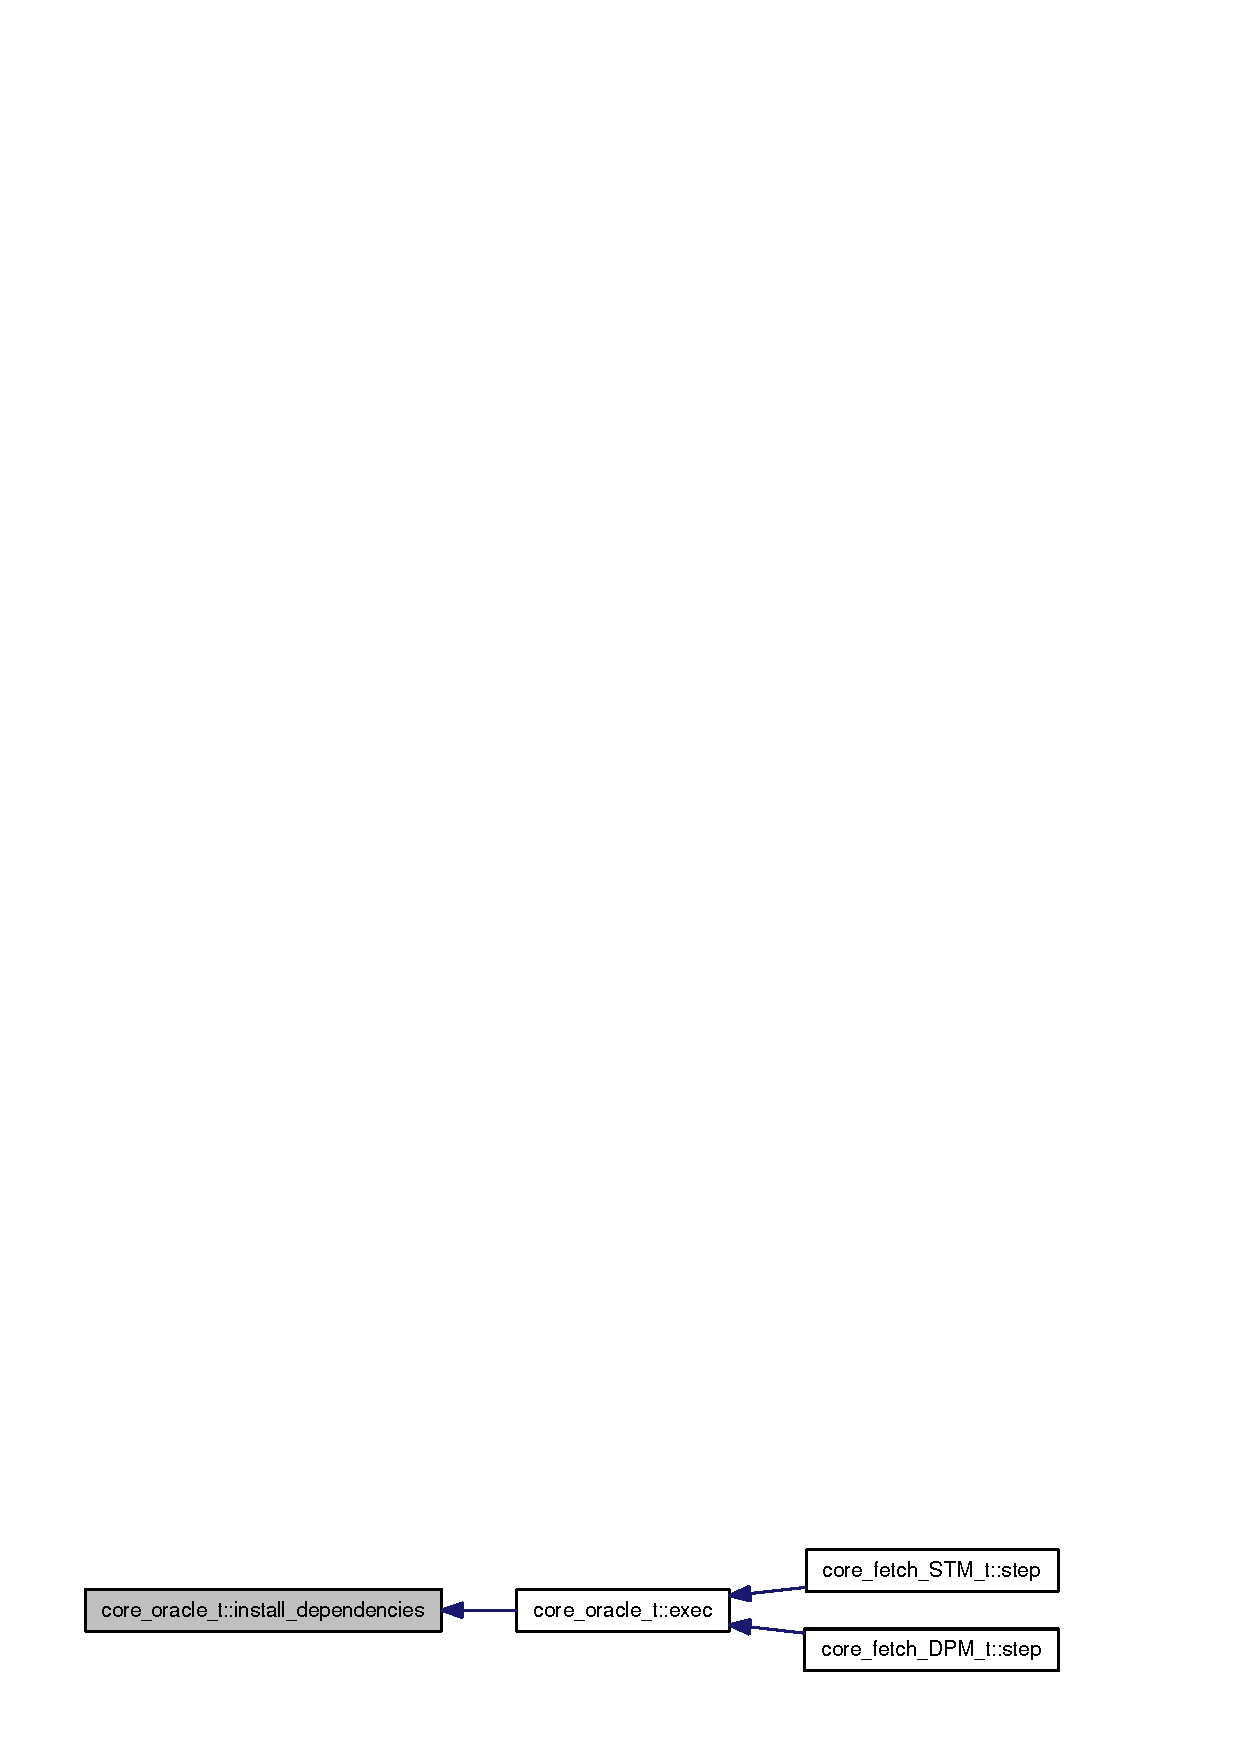
\includegraphics[width=256pt]{classcore__oracle__t_deeae95a29f95000a81b20fb895a2e64_icgraph}
\end{center}
\end{figure}
\index{core\_\-oracle\_\-t@{core\_\-oracle\_\-t}!install\_\-mapping@{install\_\-mapping}}
\index{install\_\-mapping@{install\_\-mapping}!core_oracle_t@{core\_\-oracle\_\-t}}
\subsubsection[{install\_\-mapping}]{\setlength{\rightskip}{0pt plus 5cm}void core\_\-oracle\_\-t::install\_\-mapping (struct {\bf uop\_\-t} $\ast$const  {\em uop})\hspace{0.3cm}{\tt  [protected]}}\label{classcore__oracle__t_8a47de2d0fbb812311a55d1204cdc1c1}




Definition at line 1906 of file zesto-oracle.cpp.

References DCREG, uop\_\-t::decode, dep\_\-map, DGPR, DNA, get\_\-map\_\-node(), MD\_\-REG\_\-AFLAGS, MD\_\-REG\_\-ZERO, core\_\-oracle\_\-t::core\_\-oracle\_\-t::map\_\-node\_\-t::next, uop\_\-t::odep\_\-name, uop\_\-t::oflags, core\_\-oracle\_\-t::core\_\-oracle\_\-t::map\_\-node\_\-t::prev, and core\_\-oracle\_\-t::core\_\-oracle\_\-t::map\_\-node\_\-t::uop.

Referenced by exec().

Here is the caller graph for this function:\nopagebreak
\begin{figure}[H]
\begin{center}
\leavevmode
\includegraphics[width=244pt]{classcore__oracle__t_8a47de2d0fbb812311a55d1204cdc1c1_icgraph}
\end{center}
\end{figure}
\index{core\_\-oracle\_\-t@{core\_\-oracle\_\-t}!next\_\-index@{next\_\-index}}
\index{next\_\-index@{next\_\-index}!core_oracle_t@{core\_\-oracle\_\-t}}
\subsubsection[{next\_\-index}]{\setlength{\rightskip}{0pt plus 5cm}int core\_\-oracle\_\-t::next\_\-index (const int {\em index})}\label{classcore__oracle__t_3d8ea00f353d569980869333b7a92668}




Definition at line 345 of file zesto-oracle.cpp.

References modinc(), and MopQ\_\-size.

Referenced by core\_\-fetch\_\-STM\_\-t::Mop\_\-consume(), and core\_\-fetch\_\-DPM\_\-t::step().

Here is the caller graph for this function:\nopagebreak
\begin{figure}[H]
\begin{center}
\leavevmode
\includegraphics[width=187pt]{classcore__oracle__t_3d8ea00f353d569980869333b7a92668_icgraph}
\end{center}
\end{figure}
\index{core\_\-oracle\_\-t@{core\_\-oracle\_\-t}!pipe\_\-flush@{pipe\_\-flush}}
\index{pipe\_\-flush@{pipe\_\-flush}!core_oracle_t@{core\_\-oracle\_\-t}}
\subsubsection[{pipe\_\-flush}]{\setlength{\rightskip}{0pt plus 5cm}void core\_\-oracle\_\-t::pipe\_\-flush (struct {\bf Mop\_\-t} $\ast$const  {\em Mop})}\label{classcore__oracle__t_d79ed0d31e9421037f71a3aae2aa0cbb}




Definition at line 1716 of file zesto-oracle.cpp.

References Mop\_\-t::core, core\_\-t::current\_\-thread, Mop\_\-t::fetch, core\_\-t::id, md\_\-fetch\_\-next\_\-pc(), moddec(), MopQ, MopQ\_\-head, MopQ\_\-num, MopQ\_\-size, Mop\_\-t::NextPC, Mop\_\-t::oracle, pipe\_\-recover(), Mop\_\-t::pred\_\-NPC, thread\_\-t::regs, regs\_\-t::regs\_\-NPC, spec\_\-mode, store\_\-nextPC, and zesto\_\-assert.

Referenced by core\_\-exec\_\-DPM\_\-t::ALU\_\-exec(), and core\_\-exec\_\-DPM\_\-t::LDST\_\-exec().

Here is the caller graph for this function:\nopagebreak
\begin{figure}[H]
\begin{center}
\leavevmode
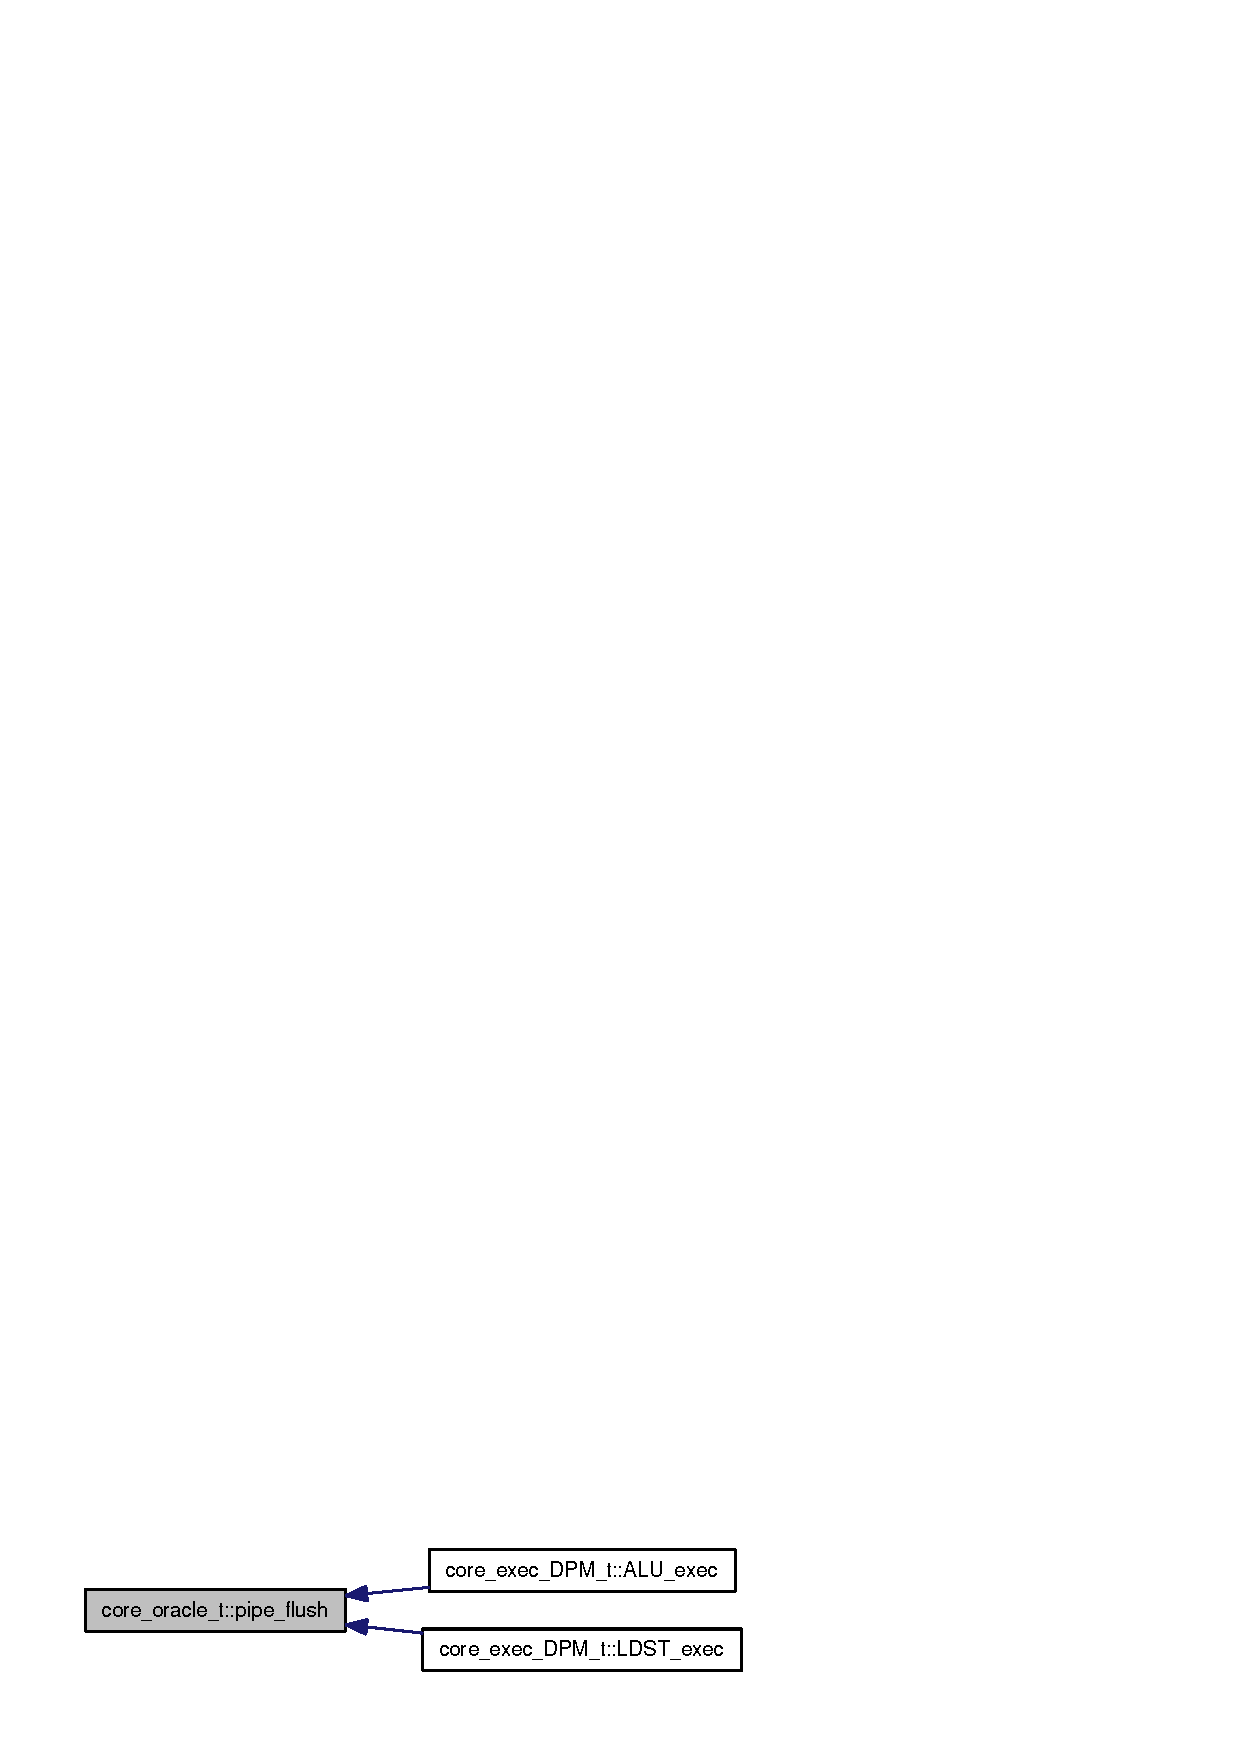
\includegraphics[width=180pt]{classcore__oracle__t_d79ed0d31e9421037f71a3aae2aa0cbb_icgraph}
\end{center}
\end{figure}
\index{core\_\-oracle\_\-t@{core\_\-oracle\_\-t}!pipe\_\-recover@{pipe\_\-recover}}
\index{pipe\_\-recover@{pipe\_\-recover}!core_oracle_t@{core\_\-oracle\_\-t}}
\subsubsection[{pipe\_\-recover}]{\setlength{\rightskip}{0pt plus 5cm}void core\_\-oracle\_\-t::pipe\_\-recover (struct {\bf Mop\_\-t} $\ast$const  {\em Mop}, \/  const {\bf md\_\-addr\_\-t} {\em New\_\-PC})}\label{classcore__oracle__t_c687f6e9c8564e5fd108ca8c9f771dce}




Definition at line 1696 of file zesto-oracle.cpp.

References core\_\-t::alloc, core\_\-fetch\_\-t::bpred, Mop\_\-t::bpred\_\-update, core\_\-t::commit, core, core\_\-t::decode, core\_\-t::exec, Mop\_\-t::fetch, core\_\-t::fetch, core\_\-knobs\_\-t::fetch, Mop\_\-t::inst, core\_\-knobs\_\-t::jeclear\_\-delay, core\_\-fetch\_\-t::jeclear\_\-enqueue(), core\_\-t::knobs, knobs, md\_\-inst\_\-t::len, Mop\_\-t::PC, core\_\-fetch\_\-t::recover(), core\_\-decode\_\-t::recover(), core\_\-alloc\_\-t::recover(), core\_\-exec\_\-t::recover(), core\_\-commit\_\-t::recover(), recover(), and bpred\_\-t::recover().

Referenced by core\_\-exec\_\-STM\_\-t::ALU\_\-exec(), core\_\-exec\_\-DPM\_\-t::ALU\_\-exec(), core\_\-exec\_\-DPM\_\-t::LDQ\_\-schedule(), core\_\-exec\_\-STM\_\-t::LDST\_\-exec(), core\_\-exec\_\-DPM\_\-t::LDST\_\-exec(), core\_\-exec\_\-STM\_\-t::load\_\-writeback(), core\_\-exec\_\-DPM\_\-t::load\_\-writeback(), and pipe\_\-flush().

Here is the caller graph for this function:\nopagebreak
\begin{figure}[H]
\begin{center}
\leavevmode
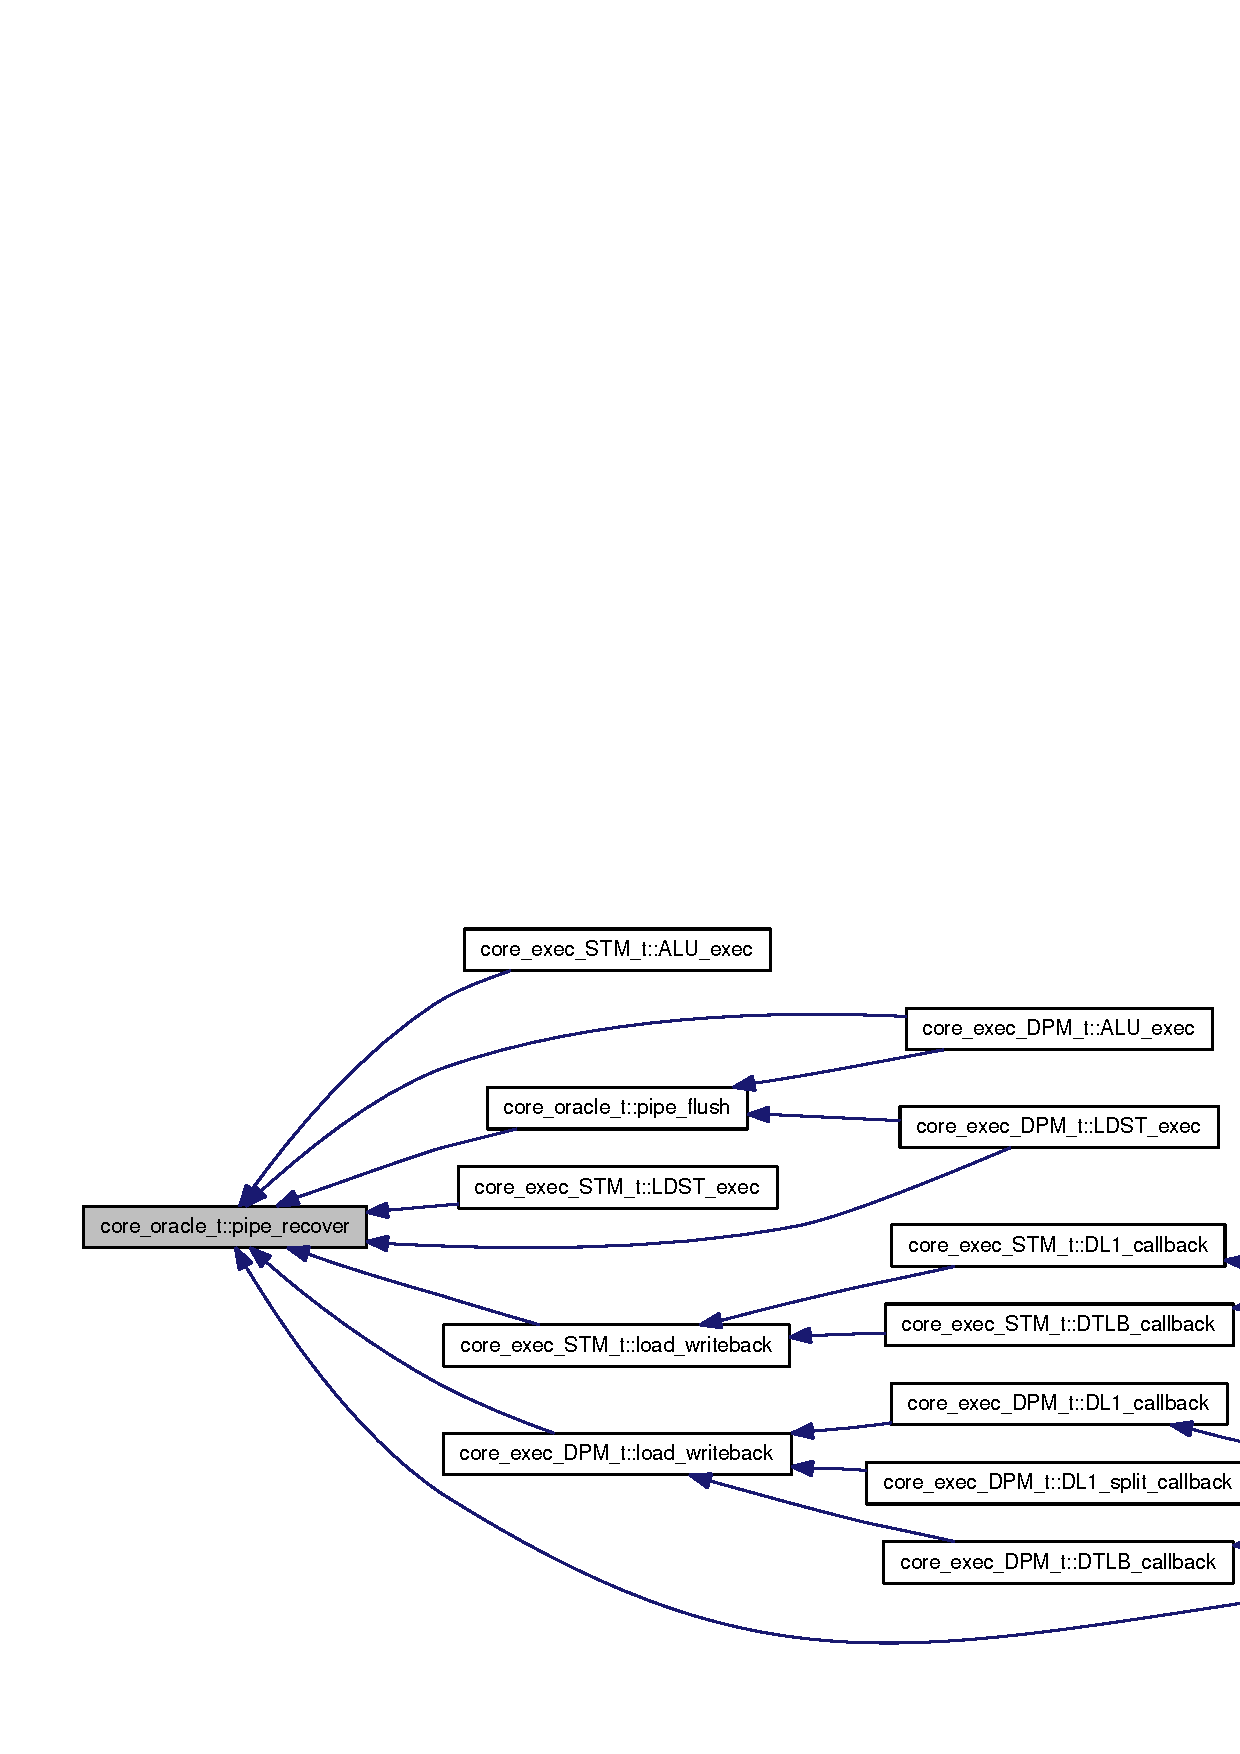
\includegraphics[width=403pt]{classcore__oracle__t_c687f6e9c8564e5fd108ca8c9f771dce_icgraph}
\end{center}
\end{figure}
\index{core\_\-oracle\_\-t@{core\_\-oracle\_\-t}!recover@{recover}}
\index{recover@{recover}!core_oracle_t@{core\_\-oracle\_\-t}}
\subsubsection[{recover}]{\setlength{\rightskip}{0pt plus 5cm}void core\_\-oracle\_\-t::recover (const struct {\bf Mop\_\-t} $\ast$const  {\em Mop})}\label{classcore__oracle__t_3262388e107011060f8fe40023f235c5}




Definition at line 1658 of file zesto-oracle.cpp.

References core\_\-fetch\_\-t::bpred, Mop\_\-t::bpred\_\-update, Mop\_\-t::branch\_\-mispred, core, current\_\-Mop, core\_\-t::current\_\-thread, fatal(), Mop\_\-t::fetch, core\_\-t::fetch, bpred\_\-t::flush(), moddec(), MopQ, MopQ\_\-head, MopQ\_\-num, MopQ\_\-size, MopQ\_\-tail, Mop\_\-t::NextPC, Mop\_\-t::oracle, Mop\_\-t::PC, thread\_\-t::regs, regs\_\-t::regs\_\-NPC, regs\_\-t::regs\_\-PC, bpred\_\-t::return\_\-state\_\-cache(), Mop\_\-t::spec\_\-mode, spec\_\-mode, undo(), and Mop\_\-t::valid.

Referenced by core\_\-decode\_\-STM\_\-t::check\_\-target(), core\_\-decode\_\-DPM\_\-t::check\_\-target(), pipe\_\-recover(), and core\_\-fetch\_\-DPM\_\-t::step().

Here is the caller graph for this function:\nopagebreak
\begin{figure}[H]
\begin{center}
\leavevmode
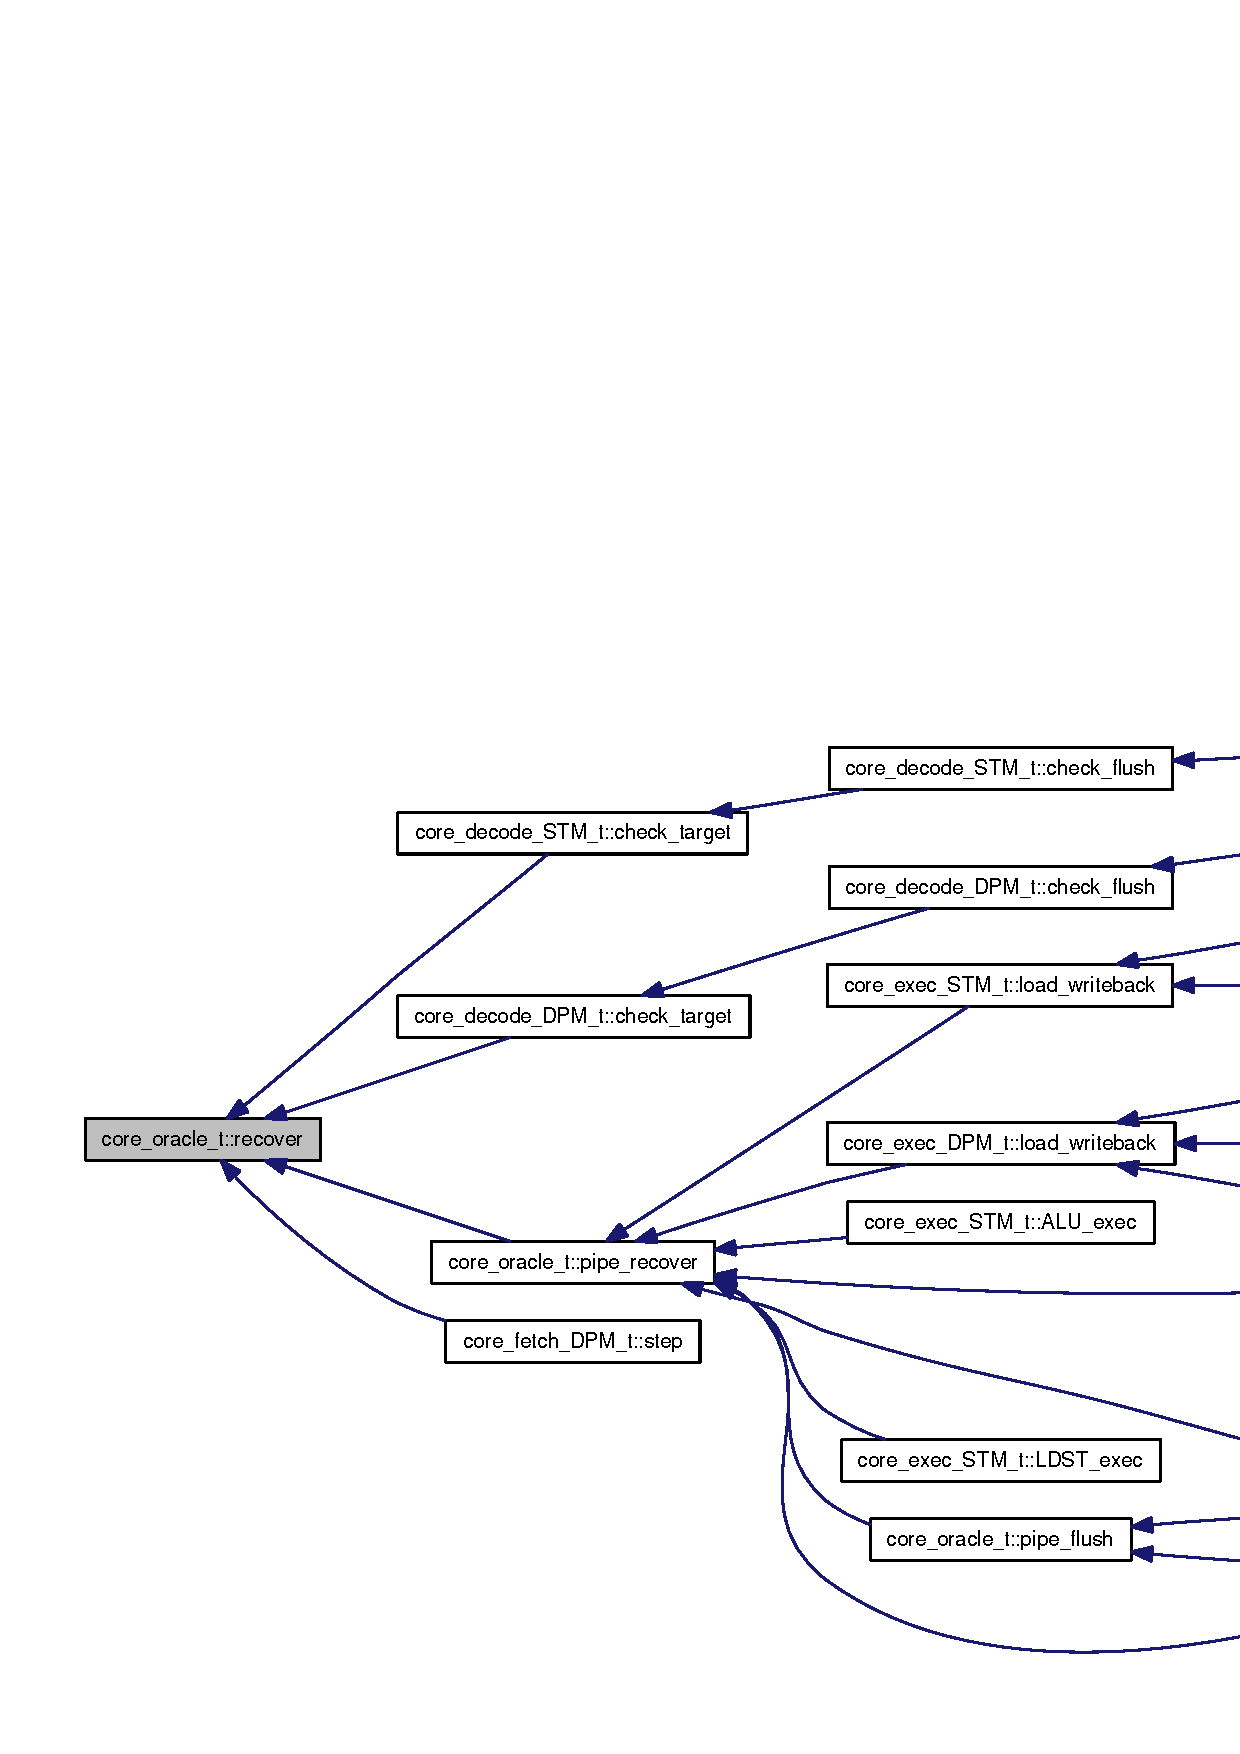
\includegraphics[width=420pt]{classcore__oracle__t_3262388e107011060f8fe40023f235c5_icgraph}
\end{center}
\end{figure}
\index{core\_\-oracle\_\-t@{core\_\-oracle\_\-t}!reg\_\-stats@{reg\_\-stats}}
\index{reg\_\-stats@{reg\_\-stats}!core_oracle_t@{core\_\-oracle\_\-t}}
\subsubsection[{reg\_\-stats}]{\setlength{\rightskip}{0pt plus 5cm}void core\_\-oracle\_\-t::reg\_\-stats (struct {\bf stat\_\-sdb\_\-t} $\ast$const  {\em sdb})}\label{classcore__oracle__t_7d71b6dc91df7d7d00820e3aea46f576}




Definition at line 224 of file zesto-oracle.cpp.

References core, core\_\-t::current\_\-thread, thread\_\-t::id, core\_\-t::core\_\-t::core\_\-stat\_\-t::MopQ\_\-full\_\-cycles, core\_\-t::core\_\-t::core\_\-stat\_\-t::MopQ\_\-occupancy, core\_\-t::num\_\-emergency\_\-recoveries, core\_\-t::core\_\-t::core\_\-stat\_\-t::oracle\_\-bogus\_\-cycles, core\_\-t::core\_\-t::core\_\-stat\_\-t::oracle\_\-eff\_\-uop\_\-undo, core\_\-t::core\_\-t::core\_\-stat\_\-t::oracle\_\-inst\_\-undo, core\_\-t::core\_\-t::core\_\-stat\_\-t::oracle\_\-num\_\-branches, core\_\-t::core\_\-t::core\_\-stat\_\-t::oracle\_\-num\_\-loads, core\_\-t::core\_\-t::core\_\-stat\_\-t::oracle\_\-num\_\-refs, core\_\-t::core\_\-t::core\_\-stat\_\-t::oracle\_\-total\_\-branches, core\_\-t::core\_\-t::core\_\-stat\_\-t::oracle\_\-total\_\-eff\_\-uops, core\_\-t::core\_\-t::core\_\-stat\_\-t::oracle\_\-total\_\-insn, core\_\-t::core\_\-t::core\_\-stat\_\-t::oracle\_\-total\_\-loads, core\_\-t::core\_\-t::core\_\-stat\_\-t::oracle\_\-total\_\-refs, core\_\-t::core\_\-t::core\_\-stat\_\-t::oracle\_\-total\_\-uops, core\_\-t::core\_\-t::core\_\-stat\_\-t::oracle\_\-uop\_\-undo, core\_\-t::stat, stat\_\-reg\_\-counter, stat\_\-reg\_\-formula(), stat\_\-reg\_\-note(), and syscall\_\-mem\_\-accesses.\index{core\_\-oracle\_\-t@{core\_\-oracle\_\-t}!reset\_\-execution@{reset\_\-execution}}
\index{reset\_\-execution@{reset\_\-execution}!core_oracle_t@{core\_\-oracle\_\-t}}
\subsubsection[{reset\_\-execution}]{\setlength{\rightskip}{0pt plus 5cm}void core\_\-oracle\_\-t::reset\_\-execution (void)}\label{classcore__oracle__t_cd307b32aa377a56b3f4dc79b2122038}




Definition at line 1781 of file zesto-oracle.cpp.

References core\_\-t::alloc, core\_\-fetch\_\-t::bogus, core\_\-t::commit, complete\_\-flush(), core, core\_\-t::current\_\-thread, core\_\-t::decode, core\_\-t::exec, core\_\-t::fetch, core\_\-t::core\_\-t::core\_\-stat\_\-t::oracle\_\-resets, core\_\-fetch\_\-t::PC, core\_\-fetch\_\-t::recover(), core\_\-decode\_\-t::recover(), core\_\-alloc\_\-t::recover(), core\_\-exec\_\-t::recover(), core\_\-commit\_\-t::recover(), thread\_\-t::regs, regs\_\-t::regs\_\-PC, and core\_\-t::stat.

Referenced by core\_\-commit\_\-STM\_\-t::step(), and core\_\-commit\_\-DPM\_\-t::step().

Here is the caller graph for this function:\nopagebreak
\begin{figure}[H]
\begin{center}
\leavevmode
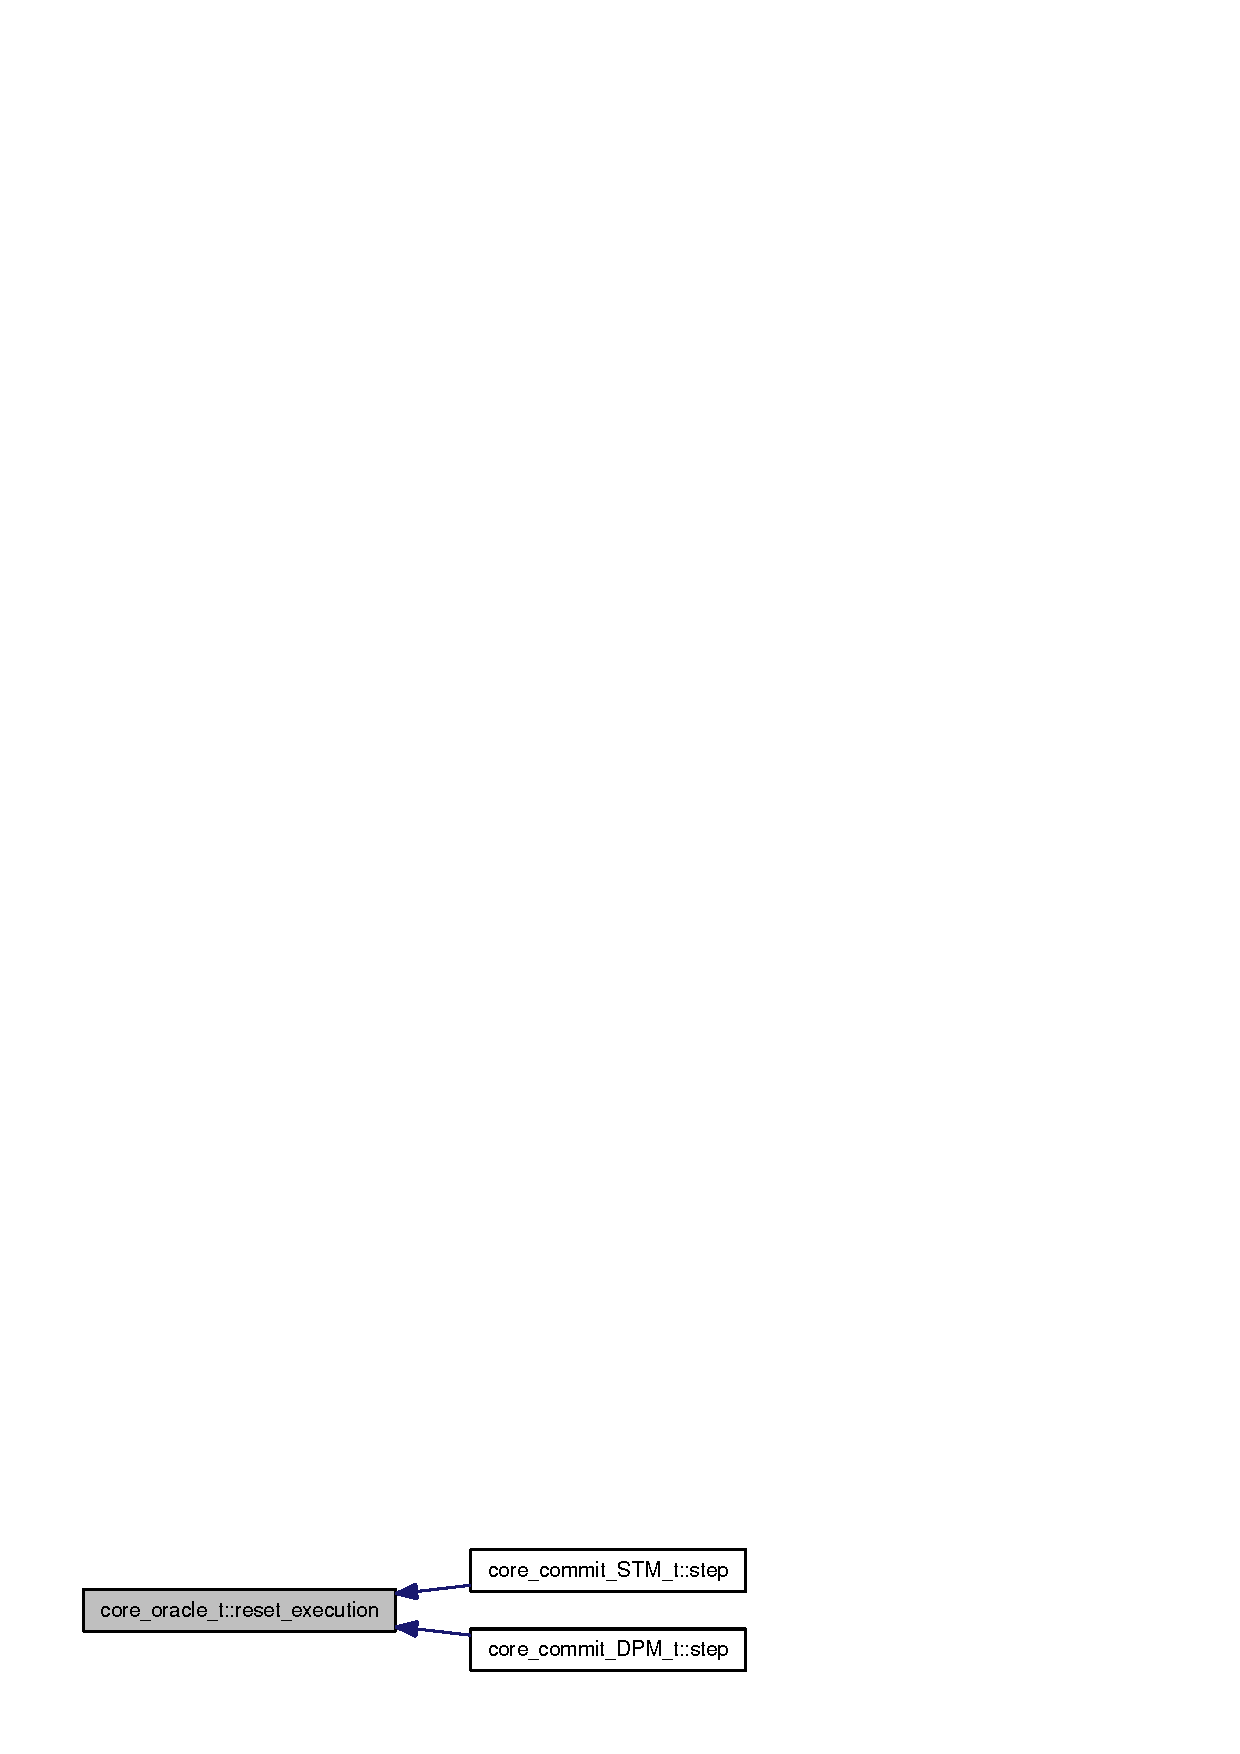
\includegraphics[width=181pt]{classcore__oracle__t_cd307b32aa377a56b3f4dc79b2122038_icgraph}
\end{center}
\end{figure}
\index{core\_\-oracle\_\-t@{core\_\-oracle\_\-t}!return\_\-map\_\-node@{return\_\-map\_\-node}}
\index{return\_\-map\_\-node@{return\_\-map\_\-node}!core_oracle_t@{core\_\-oracle\_\-t}}
\subsubsection[{return\_\-map\_\-node}]{\setlength{\rightskip}{0pt plus 5cm}void core\_\-oracle\_\-t::return\_\-map\_\-node (struct {\bf map\_\-node\_\-t} $\ast$const  {\em p})\hspace{0.3cm}{\tt  [protected]}}\label{classcore__oracle__t_6ed0bc2ff222597a87894e8fe6d53fc1}




Definition at line 2035 of file zesto-oracle.cpp.

References map\_\-free\_\-pool, map\_\-free\_\-pool\_\-debt, core\_\-oracle\_\-t::core\_\-oracle\_\-t::map\_\-node\_\-t::next, core\_\-oracle\_\-t::core\_\-oracle\_\-t::map\_\-node\_\-t::prev, and core\_\-oracle\_\-t::core\_\-oracle\_\-t::map\_\-node\_\-t::uop.

Referenced by commit\_\-mapping(), and undo\_\-mapping().

Here is the caller graph for this function:\nopagebreak
\begin{figure}[H]
\begin{center}
\leavevmode
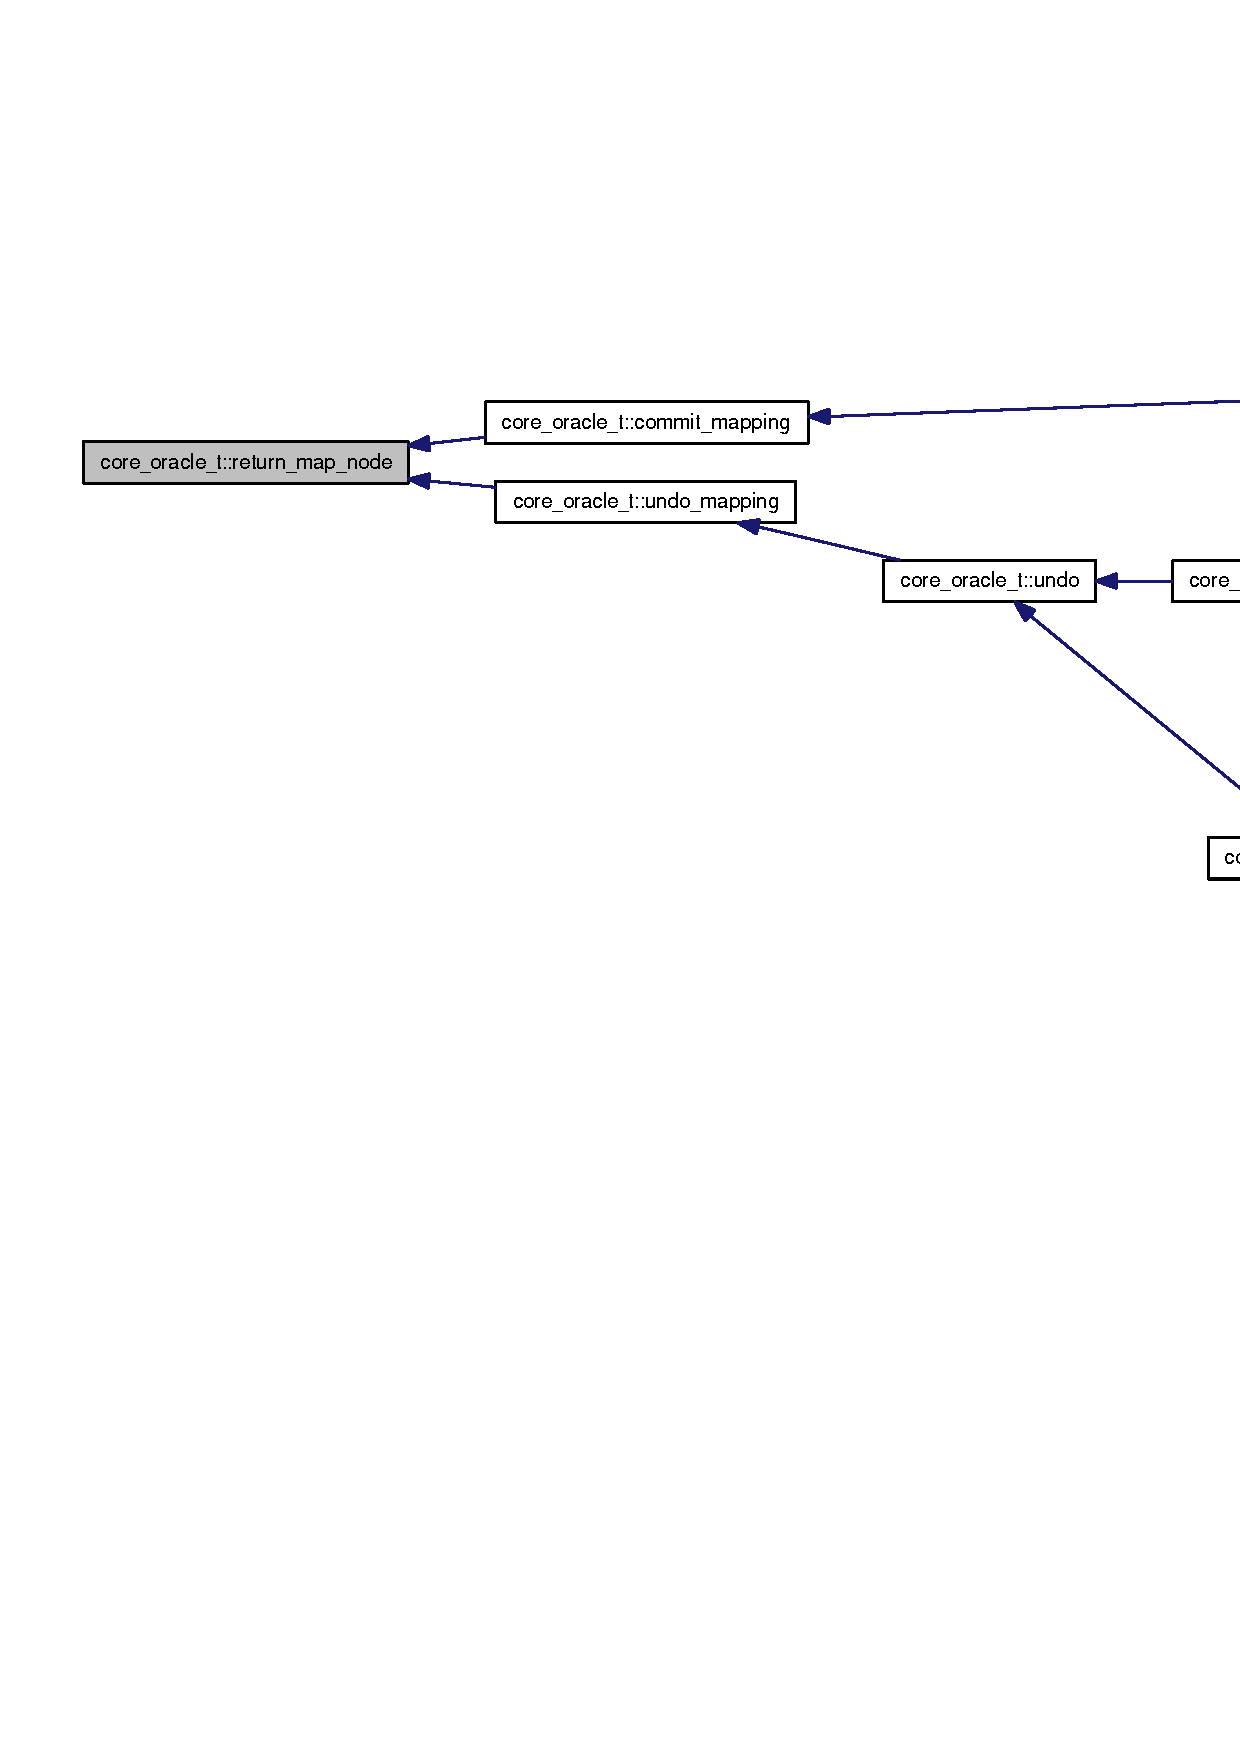
\includegraphics[width=420pt]{classcore__oracle__t_6ed0bc2ff222597a87894e8fe6d53fc1_icgraph}
\end{center}
\end{figure}
\index{core\_\-oracle\_\-t@{core\_\-oracle\_\-t}!return\_\-spec\_\-mem\_\-node@{return\_\-spec\_\-mem\_\-node}}
\index{return\_\-spec\_\-mem\_\-node@{return\_\-spec\_\-mem\_\-node}!core_oracle_t@{core\_\-oracle\_\-t}}
\subsubsection[{return\_\-spec\_\-mem\_\-node}]{\setlength{\rightskip}{0pt plus 5cm}void core\_\-oracle\_\-t::return\_\-spec\_\-mem\_\-node (struct {\bf spec\_\-byte\_\-t} $\ast$const  {\em p})\hspace{0.3cm}{\tt  [protected]}}\label{classcore__oracle__t_ecb0129c38db27a8d8424d8171025145}




Definition at line 2170 of file zesto-oracle.cpp.

References spec\_\-byte\_\-t::addr, spec\_\-byte\_\-t::next, spec\_\-byte\_\-t::prev, spec\_\-mem\_\-free\_\-pool, and spec\_\-byte\_\-t::val.

Referenced by commit\_\-write\_\-byte(), and squash\_\-write\_\-byte().

Here is the caller graph for this function:\nopagebreak
\begin{figure}[H]
\begin{center}
\leavevmode
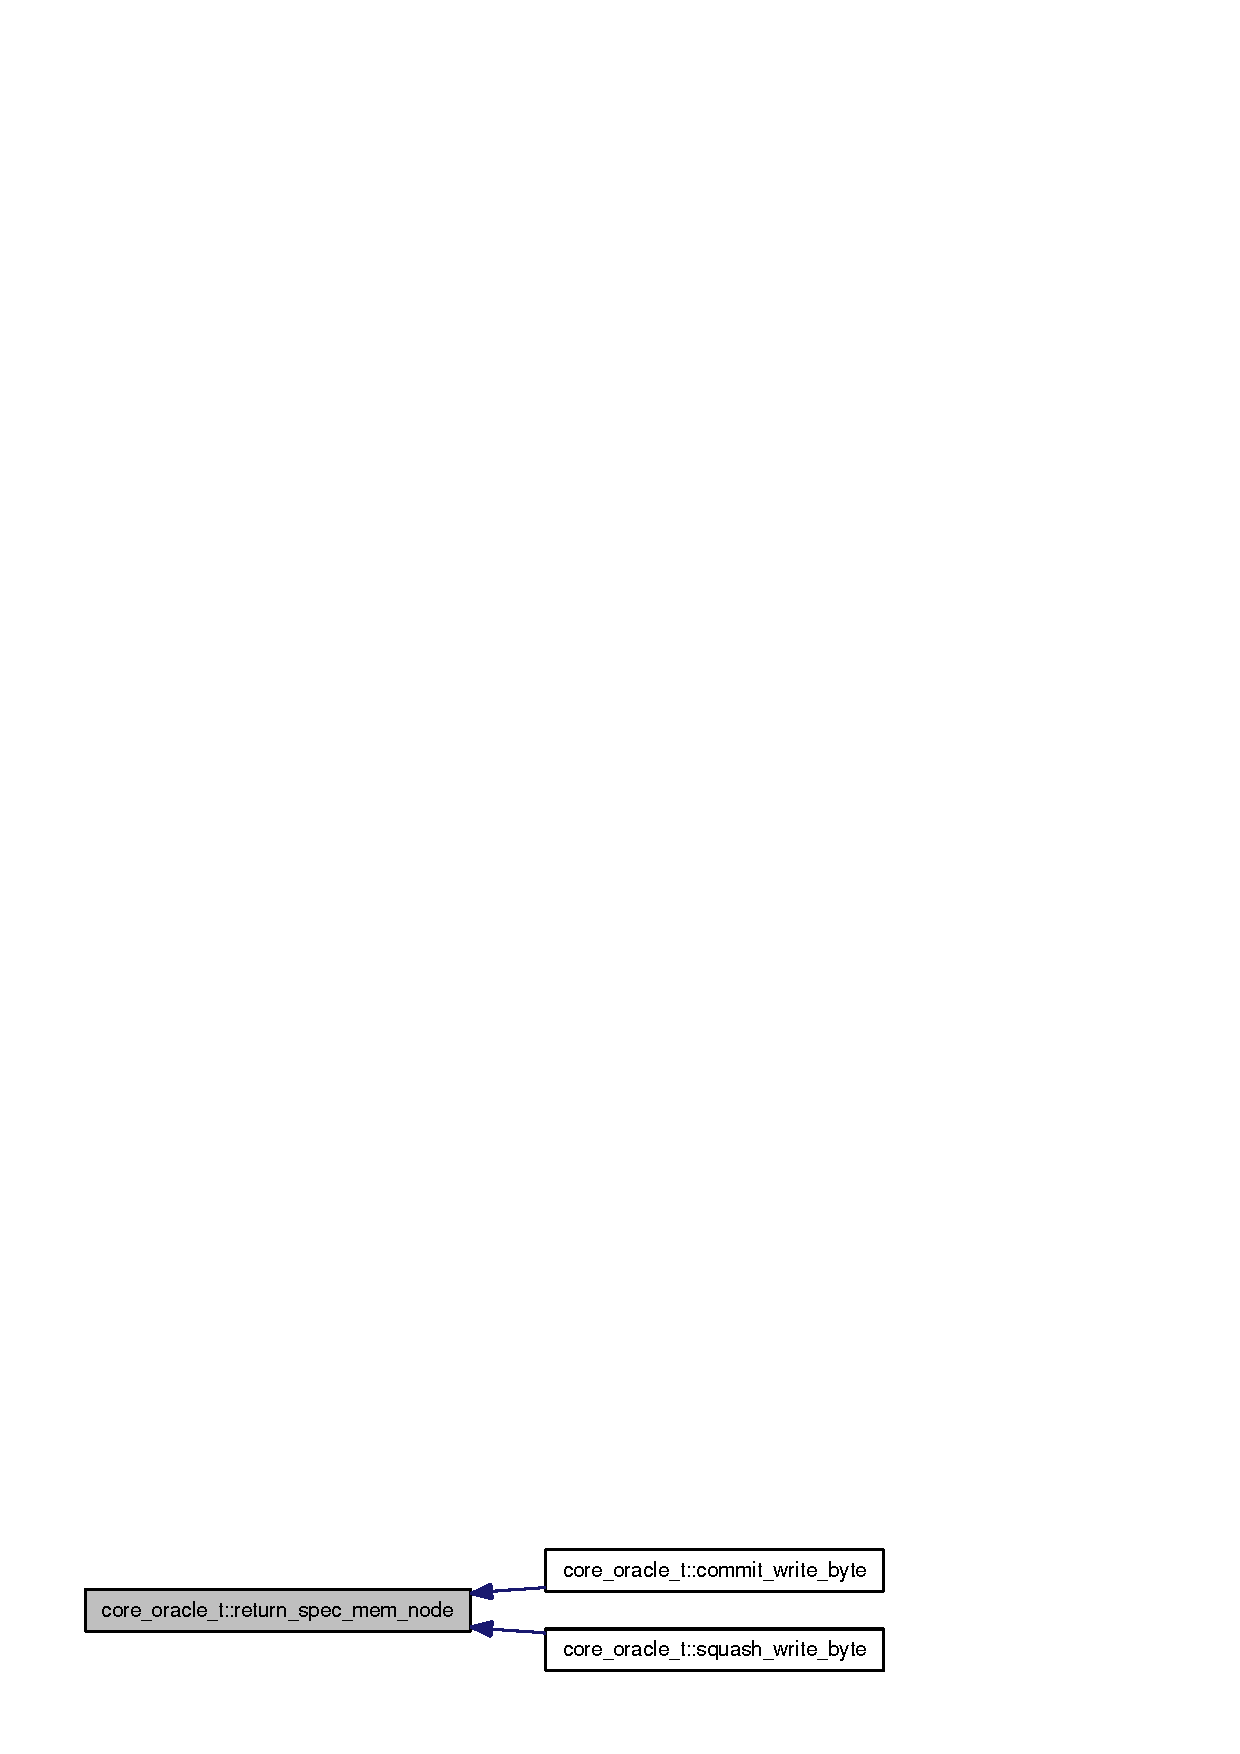
\includegraphics[width=214pt]{classcore__oracle__t_ecb0129c38db27a8d8424d8171025145_icgraph}
\end{center}
\end{figure}
\index{core\_\-oracle\_\-t@{core\_\-oracle\_\-t}!spec\_\-read\_\-byte@{spec\_\-read\_\-byte}}
\index{spec\_\-read\_\-byte@{spec\_\-read\_\-byte}!core_oracle_t@{core\_\-oracle\_\-t}}
\subsubsection[{spec\_\-read\_\-byte}]{\setlength{\rightskip}{0pt plus 5cm}bool core\_\-oracle\_\-t::spec\_\-read\_\-byte (const {\bf md\_\-addr\_\-t} {\em addr}, \/  {\bf byte\_\-t} $\ast$const  {\em valp})}\label{classcore__oracle__t_24e69274c807607f5ef86295f46eafbf}




Definition at line 372 of file zesto-oracle.cpp.

References spec\_\-byte\_\-t::addr, core\_\-oracle\_\-t::core\_\-oracle\_\-t::spec\_\-mem\_\-t::hash, MEM\_\-HASH\_\-MASK, spec\_\-byte\_\-t::prev, spec\_\-mem\_\-map, core\_\-oracle\_\-t::core\_\-oracle\_\-t::spec\_\-mem\_\-t::tail, and spec\_\-byte\_\-t::val.\index{core\_\-oracle\_\-t@{core\_\-oracle\_\-t}!spec\_\-write\_\-byte@{spec\_\-write\_\-byte}}
\index{spec\_\-write\_\-byte@{spec\_\-write\_\-byte}!core_oracle_t@{core\_\-oracle\_\-t}}
\subsubsection[{spec\_\-write\_\-byte}]{\setlength{\rightskip}{0pt plus 5cm}struct {\bf spec\_\-byte\_\-t} $\ast$ core\_\-oracle\_\-t::spec\_\-write\_\-byte (const {\bf md\_\-addr\_\-t} {\em addr}, \/  const {\bf byte\_\-t} {\em val})\hspace{0.3cm}{\tt  [read]}}\label{classcore__oracle__t_f60392fcde2b50e69bf96ef7fa845463}




Definition at line 352 of file zesto-oracle.cpp.

References spec\_\-byte\_\-t::addr, get\_\-spec\_\-mem\_\-node(), core\_\-oracle\_\-t::core\_\-oracle\_\-t::spec\_\-mem\_\-t::hash, core\_\-oracle\_\-t::core\_\-oracle\_\-t::spec\_\-mem\_\-t::head, MEM\_\-HASH\_\-MASK, spec\_\-byte\_\-t::next, spec\_\-byte\_\-t::prev, spec\_\-mem\_\-map, core\_\-oracle\_\-t::core\_\-oracle\_\-t::spec\_\-mem\_\-t::tail, and spec\_\-byte\_\-t::val.\index{core\_\-oracle\_\-t@{core\_\-oracle\_\-t}!squash\_\-write\_\-byte@{squash\_\-write\_\-byte}}
\index{squash\_\-write\_\-byte@{squash\_\-write\_\-byte}!core_oracle_t@{core\_\-oracle\_\-t}}
\subsubsection[{squash\_\-write\_\-byte}]{\setlength{\rightskip}{0pt plus 5cm}void core\_\-oracle\_\-t::squash\_\-write\_\-byte (struct {\bf spec\_\-byte\_\-t} $\ast$const  {\em p})\hspace{0.3cm}{\tt  [protected]}}\label{classcore__oracle__t_e14bba8a8cf6ecfc9a52845e3c1760aa}




Definition at line 2182 of file zesto-oracle.cpp.

References spec\_\-byte\_\-t::addr, core\_\-oracle\_\-t::core\_\-oracle\_\-t::spec\_\-mem\_\-t::hash, core\_\-oracle\_\-t::core\_\-oracle\_\-t::spec\_\-mem\_\-t::head, MEM\_\-HASH\_\-MASK, spec\_\-byte\_\-t::next, spec\_\-byte\_\-t::prev, return\_\-spec\_\-mem\_\-node(), spec\_\-mem\_\-map, and core\_\-oracle\_\-t::core\_\-oracle\_\-t::spec\_\-mem\_\-t::tail.\index{core\_\-oracle\_\-t@{core\_\-oracle\_\-t}!syscall\_\-callback@{syscall\_\-callback}}
\index{syscall\_\-callback@{syscall\_\-callback}!core_oracle_t@{core\_\-oracle\_\-t}}
\subsubsection[{syscall\_\-callback}]{\setlength{\rightskip}{0pt plus 5cm}void core\_\-oracle\_\-t::syscall\_\-callback (void $\ast$const  {\em op})\hspace{0.3cm}{\tt  [static, protected]}}\label{classcore__oracle__t_0f8c8d4e3eb748b911028d64d2a086d8}




Definition at line 464 of file zesto-oracle.cpp.\index{core\_\-oracle\_\-t@{core\_\-oracle\_\-t}!syscall\_\-get\_\-action\_\-id@{syscall\_\-get\_\-action\_\-id}}
\index{syscall\_\-get\_\-action\_\-id@{syscall\_\-get\_\-action\_\-id}!core_oracle_t@{core\_\-oracle\_\-t}}
\subsubsection[{syscall\_\-get\_\-action\_\-id}]{\setlength{\rightskip}{0pt plus 5cm}{\bf seq\_\-t} core\_\-oracle\_\-t::syscall\_\-get\_\-action\_\-id (void $\ast$const  {\em op})\hspace{0.3cm}{\tt  [static, protected]}}\label{classcore__oracle__t_16826da0aea8695f558397af8c0be45b}




Definition at line 474 of file zesto-oracle.cpp.

References DUMMY\_\-SYSCALL\_\-ACTION\_\-ID.\index{core\_\-oracle\_\-t@{core\_\-oracle\_\-t}!syscall\_\-mem\_\-access@{syscall\_\-mem\_\-access}}
\index{syscall\_\-mem\_\-access@{syscall\_\-mem\_\-access}!core_oracle_t@{core\_\-oracle\_\-t}}
\subsubsection[{syscall\_\-mem\_\-access}]{\setlength{\rightskip}{0pt plus 5cm}enum {\bf md\_\-fault\_\-type} core\_\-oracle\_\-t::syscall\_\-mem\_\-access (int {\em thread\_\-id}, \/  struct {\bf mem\_\-t} $\ast$ {\em mem}, \/  enum {\bf mem\_\-cmd} {\em cmd}, \/  {\bf md\_\-addr\_\-t} {\em addr}, \/  void $\ast$ {\em vp}, \/  int {\em nbytes})\hspace{0.3cm}{\tt  [static]}}\label{classcore__oracle__t_e266894eeb549a7421ac488d9b18edaf}




Definition at line 395 of file zesto-oracle.cpp.

References core\_\-oracle\_\-t::core\_\-oracle\_\-t::syscall\_\-mem\_\-req\_\-t::addr, CACHE\_\-READ, CACHE\_\-WRITE, core\_\-oracle\_\-t::core\_\-oracle\_\-t::syscall\_\-mem\_\-req\_\-t::cmd, core, cores, thread\_\-t::current\_\-core, fatal(), core\_\-t::knobs, mem\_\-access(), mem\_\-req\_\-free\_\-pool, core\_\-knobs\_\-t::memory, core\_\-oracle\_\-t::core\_\-oracle\_\-t::syscall\_\-mem\_\-req\_\-t::next, core\_\-t::oracle, Read, syscall\_\-mem\_\-accesses, syscall\_\-mem\_\-req\_\-head, syscall\_\-mem\_\-req\_\-tail, syscall\_\-mem\_\-reqs, core\_\-knobs\_\-t::syscall\_\-memory\_\-latency, core\_\-oracle\_\-t::core\_\-oracle\_\-t::syscall\_\-mem\_\-req\_\-t::thread\_\-id, and threads.\index{core\_\-oracle\_\-t@{core\_\-oracle\_\-t}!syscall\_\-translated\_\-callback@{syscall\_\-translated\_\-callback}}
\index{syscall\_\-translated\_\-callback@{syscall\_\-translated\_\-callback}!core_oracle_t@{core\_\-oracle\_\-t}}
\subsubsection[{syscall\_\-translated\_\-callback}]{\setlength{\rightskip}{0pt plus 5cm}bool core\_\-oracle\_\-t::syscall\_\-translated\_\-callback (void $\ast$const  {\em op}, \/  const {\bf seq\_\-t} {\em action\_\-id})\hspace{0.3cm}{\tt  [static, protected]}}\label{classcore__oracle__t_a288707f42533b1b2397e9b9b59c2e0f}




Definition at line 469 of file zesto-oracle.cpp.\index{core\_\-oracle\_\-t@{core\_\-oracle\_\-t}!undo@{undo}}
\index{undo@{undo}!core_oracle_t@{core\_\-oracle\_\-t}}
\subsubsection[{undo}]{\setlength{\rightskip}{0pt plus 5cm}void core\_\-oracle\_\-t::undo (struct {\bf Mop\_\-t} $\ast$const  {\em Mop})\hspace{0.3cm}{\tt  [protected]}}\label{classcore__oracle__t_0d7765bb5655c1dd28f758143caaa8ce}




Definition at line 1587 of file zesto-oracle.cpp.

References uop\_\-t::action\_\-id, core, core\_\-t::current\_\-thread, uop\_\-t::decode, Mop\_\-t::decode, uop\_\-t::EOM, uop\_\-t::exec, Mop\_\-t::fetch, Mop\_\-t::flow\_\-length, uop\_\-t::in\_\-fusion, uop\_\-t::is\_\-fusion\_\-head, uop\_\-t::is\_\-imm, Mop\_\-t::jeclear\_\-action\_\-id, core\_\-t::new\_\-action\_\-id(), thread\_\-t::num\_\-insn, Mop\_\-t::oracle, core\_\-t::core\_\-t::core\_\-stat\_\-t::oracle\_\-eff\_\-uop\_\-undo, core\_\-t::core\_\-t::core\_\-stat\_\-t::oracle\_\-inst\_\-undo, core\_\-t::core\_\-t::core\_\-stat\_\-t::oracle\_\-uop\_\-undo, Mop\_\-t::rep\_\-seq, thread\_\-t::rep\_\-sequence, Mop\_\-t::spec\_\-mode, core\_\-t::stat, thread\_\-t::stat, undo\_\-dependencies(), undo\_\-mapping(), Mop\_\-t::uop, and ZESTO\_\-STAT.

Referenced by complete\_\-flush(), and recover().

Here is the caller graph for this function:\nopagebreak
\begin{figure}[H]
\begin{center}
\leavevmode
\includegraphics[width=420pt]{classcore__oracle__t_0d7765bb5655c1dd28f758143caaa8ce_icgraph}
\end{center}
\end{figure}
\index{core\_\-oracle\_\-t@{core\_\-oracle\_\-t}!undo\_\-dependencies@{undo\_\-dependencies}}
\index{undo\_\-dependencies@{undo\_\-dependencies}!core_oracle_t@{core\_\-oracle\_\-t}}
\subsubsection[{undo\_\-dependencies}]{\setlength{\rightskip}{0pt plus 5cm}void core\_\-oracle\_\-t::undo\_\-dependencies (struct {\bf uop\_\-t} $\ast$const  {\em uop})\hspace{0.3cm}{\tt  [protected]}}\label{classcore__oracle__t_56379122fc2f63fc767cdf82e346b98b}




Definition at line 2105 of file zesto-oracle.cpp.

References core, uop\_\-t::idep\_\-uop, MAX\_\-IDEPS, odep\_\-t::next, uop\_\-t::odep\_\-uop, odep\_\-t::op\_\-num, uop\_\-t::oracle, core\_\-t::return\_\-odep\_\-link(), and odep\_\-t::uop.

Referenced by undo().

Here is the caller graph for this function:\nopagebreak
\begin{figure}[H]
\begin{center}
\leavevmode
\includegraphics[width=420pt]{classcore__oracle__t_56379122fc2f63fc767cdf82e346b98b_icgraph}
\end{center}
\end{figure}
\index{core\_\-oracle\_\-t@{core\_\-oracle\_\-t}!undo\_\-mapping@{undo\_\-mapping}}
\index{undo\_\-mapping@{undo\_\-mapping}!core_oracle_t@{core\_\-oracle\_\-t}}
\subsubsection[{undo\_\-mapping}]{\setlength{\rightskip}{0pt plus 5cm}void core\_\-oracle\_\-t::undo\_\-mapping (const struct {\bf uop\_\-t} $\ast$const  {\em uop})\hspace{0.3cm}{\tt  [protected]}}\label{classcore__oracle__t_dc47fe294aeba52e39f9a11276522823}




Definition at line 1959 of file zesto-oracle.cpp.

References DCREG, uop\_\-t::decode, dep\_\-map, DNA, MD\_\-REG\_\-AFLAGS, MD\_\-REG\_\-ZERO, core\_\-oracle\_\-t::core\_\-oracle\_\-t::map\_\-node\_\-t::next, uop\_\-t::odep\_\-name, uop\_\-t::oflags, core\_\-oracle\_\-t::core\_\-oracle\_\-t::map\_\-node\_\-t::prev, return\_\-map\_\-node(), and core\_\-oracle\_\-t::core\_\-oracle\_\-t::map\_\-node\_\-t::uop.

Referenced by undo().

Here is the caller graph for this function:\nopagebreak
\begin{figure}[H]
\begin{center}
\leavevmode
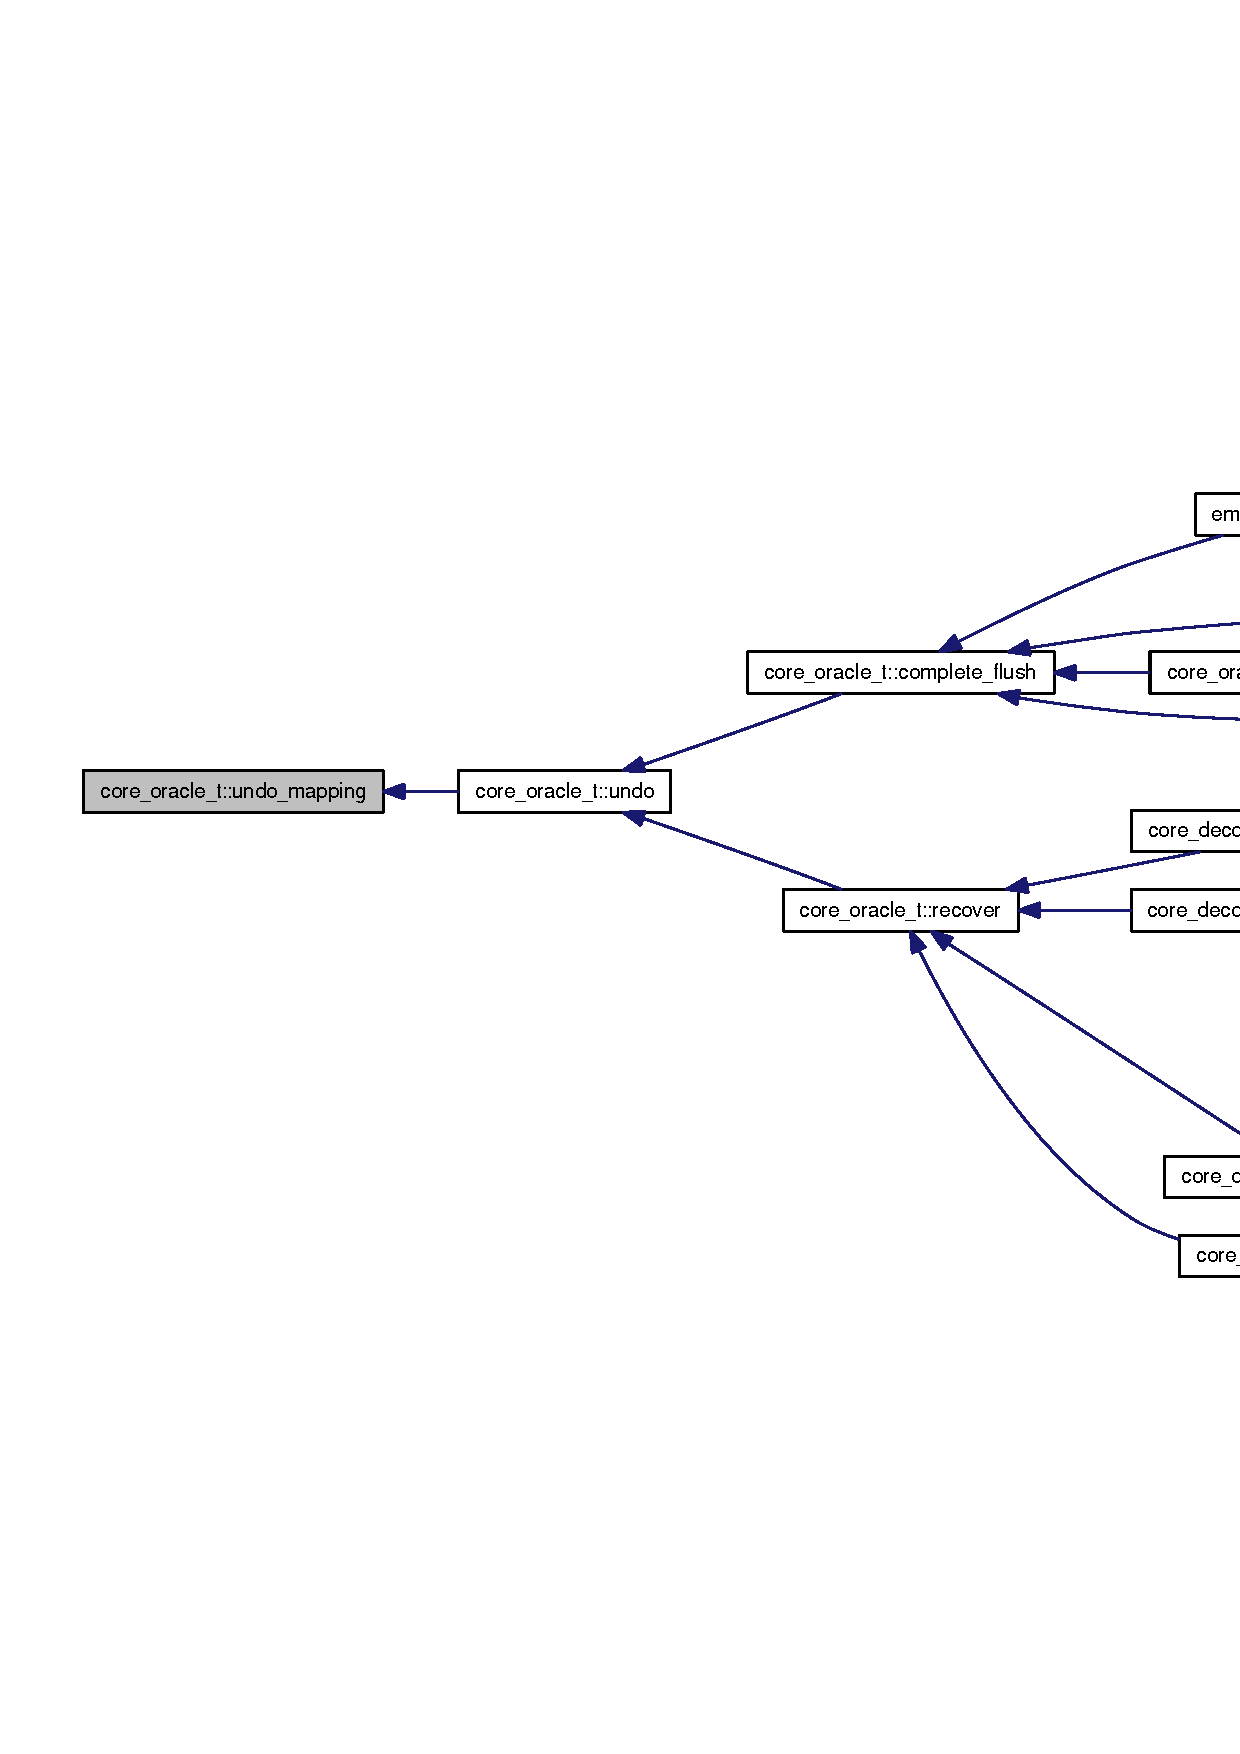
\includegraphics[width=420pt]{classcore__oracle__t_dc47fe294aeba52e39f9a11276522823_icgraph}
\end{center}
\end{figure}
\index{core\_\-oracle\_\-t@{core\_\-oracle\_\-t}!update\_\-occupancy@{update\_\-occupancy}}
\index{update\_\-occupancy@{update\_\-occupancy}!core_oracle_t@{core\_\-oracle\_\-t}}
\subsubsection[{update\_\-occupancy}]{\setlength{\rightskip}{0pt plus 5cm}void core\_\-oracle\_\-t::update\_\-occupancy (void)}\label{classcore__oracle__t_494a10decdeba4a3f043cce0186d806a}




Definition at line 327 of file zesto-oracle.cpp.

References core, core\_\-t::core\_\-t::core\_\-stat\_\-t::MopQ\_\-full\_\-cycles, MopQ\_\-num, core\_\-t::core\_\-t::core\_\-stat\_\-t::MopQ\_\-occupancy, MopQ\_\-size, and core\_\-t::stat.

Referenced by zesto\_\-component::downtick\_\-handler().

Here is the caller graph for this function:\nopagebreak
\begin{figure}[H]
\begin{center}
\leavevmode
\includegraphics[width=352pt]{classcore__oracle__t_494a10decdeba4a3f043cce0186d806a_icgraph}
\end{center}
\end{figure}


\subsection{Member Data Documentation}
\index{core\_\-oracle\_\-t@{core\_\-oracle\_\-t}!core@{core}}
\index{core@{core}!core_oracle_t@{core\_\-oracle\_\-t}}
\subsubsection[{core}]{\setlength{\rightskip}{0pt plus 5cm}struct {\bf core\_\-t}$\ast$ {\bf core\_\-oracle\_\-t::core}\hspace{0.3cm}{\tt  [read, protected]}}\label{classcore__oracle__t_32fd14747d2d54dc5e0bc2ba7d118364}




Definition at line 262 of file zesto-oracle.h.

Referenced by commit\_\-dependencies(), commit\_\-uop(), complete\_\-flush(), core\_\-oracle\_\-t(), exec(), install\_\-dependencies(), pipe\_\-recover(), recover(), reg\_\-stats(), reset\_\-execution(), syscall\_\-mem\_\-access(), undo(), undo\_\-dependencies(), and update\_\-occupancy().\index{core\_\-oracle\_\-t@{core\_\-oracle\_\-t}!current\_\-Mop@{current\_\-Mop}}
\index{current\_\-Mop@{current\_\-Mop}!core_oracle_t@{core\_\-oracle\_\-t}}
\subsubsection[{current\_\-Mop}]{\setlength{\rightskip}{0pt plus 5cm}struct {\bf Mop\_\-t}$\ast$ {\bf core\_\-oracle\_\-t::current\_\-Mop}\hspace{0.3cm}{\tt  [read, protected]}}\label{classcore__oracle__t_d1209b754eaf54cb0119beb43eea0929}




Definition at line 254 of file zesto-oracle.h.

Referenced by complete\_\-flush(), consume(), exec(), and recover().\index{core\_\-oracle\_\-t@{core\_\-oracle\_\-t}!dep\_\-map@{dep\_\-map}}
\index{dep\_\-map@{dep\_\-map}!core_oracle_t@{core\_\-oracle\_\-t}}
\subsubsection[{dep\_\-map}]{\setlength{\rightskip}{0pt plus 5cm}struct \{ ... \}   {\bf core\_\-oracle\_\-t::dep\_\-map}\hspace{0.3cm}{\tt  [protected]}}\label{classcore__oracle__t_dff628c0529f5ffc29965d2699adf61a}




Referenced by commit\_\-mapping(), core\_\-oracle\_\-t(), install\_\-dependencies(), install\_\-mapping(), and undo\_\-mapping().\index{core\_\-oracle\_\-t@{core\_\-oracle\_\-t}!DUMMY\_\-SYSCALL\_\-ACTION\_\-ID@{DUMMY\_\-SYSCALL\_\-ACTION\_\-ID}}
\index{DUMMY\_\-SYSCALL\_\-ACTION\_\-ID@{DUMMY\_\-SYSCALL\_\-ACTION\_\-ID}!core_oracle_t@{core\_\-oracle\_\-t}}
\subsubsection[{DUMMY\_\-SYSCALL\_\-ACTION\_\-ID}]{\setlength{\rightskip}{0pt plus 5cm}const {\bf seq\_\-t} {\bf core\_\-oracle\_\-t::DUMMY\_\-SYSCALL\_\-ACTION\_\-ID} = ULL(0x2E570515CA111D)\hspace{0.3cm}{\tt  [static, protected]}}\label{classcore__oracle__t_7ae3e4395fe930b73847748c92d269de}




Definition at line 295 of file zesto-oracle.h.

Referenced by syscall\_\-get\_\-action\_\-id().\index{core\_\-oracle\_\-t@{core\_\-oracle\_\-t}!DUMMY\_\-SYSCALL\_\-OP@{DUMMY\_\-SYSCALL\_\-OP}}
\index{DUMMY\_\-SYSCALL\_\-OP@{DUMMY\_\-SYSCALL\_\-OP}!core_oracle_t@{core\_\-oracle\_\-t}}
\subsubsection[{DUMMY\_\-SYSCALL\_\-OP}]{\setlength{\rightskip}{0pt plus 5cm}const unsigned {\bf core\_\-oracle\_\-t::DUMMY\_\-SYSCALL\_\-OP} = 0x515CA11\hspace{0.3cm}{\tt  [static, protected]}}\label{classcore__oracle__t_1b88181def235b9f82b8a32dc0503b15}




Definition at line 296 of file zesto-oracle.h.\index{core\_\-oracle\_\-t@{core\_\-oracle\_\-t}!head@{head}}
\index{head@{head}!core_oracle_t@{core\_\-oracle\_\-t}}
\subsubsection[{head}]{\setlength{\rightskip}{0pt plus 5cm}struct {\bf map\_\-node\_\-t}$\ast$ {\bf core\_\-oracle\_\-t::head}[MD\_\-TOTAL\_\-REGS]\hspace{0.3cm}{\tt  [read]}}\label{classcore__oracle__t_90b2a74b8c369dec9adcedad77ebe766}




Definition at line 266 of file zesto-oracle.h.\index{core\_\-oracle\_\-t@{core\_\-oracle\_\-t}!hosed@{hosed}}
\index{hosed@{hosed}!core_oracle_t@{core\_\-oracle\_\-t}}
\subsubsection[{hosed}]{\setlength{\rightskip}{0pt plus 5cm}bool {\bf core\_\-oracle\_\-t::hosed}}\label{classcore__oracle__t_d00e22e564a08b3912cf93f1e71a502d}




Definition at line 211 of file zesto-oracle.h.

Referenced by emergency\_\-recovery().\index{core\_\-oracle\_\-t@{core\_\-oracle\_\-t}!map\_\-free\_\-pool@{map\_\-free\_\-pool}}
\index{map\_\-free\_\-pool@{map\_\-free\_\-pool}!core_oracle_t@{core\_\-oracle\_\-t}}
\subsubsection[{map\_\-free\_\-pool}]{\setlength{\rightskip}{0pt plus 5cm}struct {\bf core\_\-oracle\_\-t::map\_\-node\_\-t} $\ast$ {\bf core\_\-oracle\_\-t::map\_\-free\_\-pool} = NULL\hspace{0.3cm}{\tt  [static, read, protected]}}\label{classcore__oracle__t_ed152af32c6f582d03ee8a88f2f399a3}




Definition at line 256 of file zesto-oracle.h.

Referenced by get\_\-map\_\-node(), and return\_\-map\_\-node().\index{core\_\-oracle\_\-t@{core\_\-oracle\_\-t}!map\_\-free\_\-pool\_\-debt@{map\_\-free\_\-pool\_\-debt}}
\index{map\_\-free\_\-pool\_\-debt@{map\_\-free\_\-pool\_\-debt}!core_oracle_t@{core\_\-oracle\_\-t}}
\subsubsection[{map\_\-free\_\-pool\_\-debt}]{\setlength{\rightskip}{0pt plus 5cm}int {\bf core\_\-oracle\_\-t::map\_\-free\_\-pool\_\-debt} = 0\hspace{0.3cm}{\tt  [static, protected]}}\label{classcore__oracle__t_2387b57848be51fa71ac1bd00797b4f9}




Definition at line 257 of file zesto-oracle.h.

Referenced by get\_\-map\_\-node(), and return\_\-map\_\-node().\index{core\_\-oracle\_\-t@{core\_\-oracle\_\-t}!mem\_\-req\_\-free\_\-pool@{mem\_\-req\_\-free\_\-pool}}
\index{mem\_\-req\_\-free\_\-pool@{mem\_\-req\_\-free\_\-pool}!core_oracle_t@{core\_\-oracle\_\-t}}
\subsubsection[{mem\_\-req\_\-free\_\-pool}]{\setlength{\rightskip}{0pt plus 5cm}struct {\bf syscall\_\-mem\_\-req\_\-t}$\ast$ {\bf core\_\-oracle\_\-t::mem\_\-req\_\-free\_\-pool}\hspace{0.3cm}{\tt  [read, protected]}}\label{classcore__oracle__t_05c50ff07efc7d5f8fbf6bbfbb492b58}




Definition at line 260 of file zesto-oracle.h.

Referenced by syscall\_\-mem\_\-access().\index{core\_\-oracle\_\-t@{core\_\-oracle\_\-t}!MopQ@{MopQ}}
\index{MopQ@{MopQ}!core_oracle_t@{core\_\-oracle\_\-t}}
\subsubsection[{MopQ}]{\setlength{\rightskip}{0pt plus 5cm}struct {\bf Mop\_\-t}$\ast$ {\bf core\_\-oracle\_\-t::MopQ}\hspace{0.3cm}{\tt  [read, protected]}}\label{classcore__oracle__t_ce39de7d819c6a08c18fce9294162dad}




Definition at line 249 of file zesto-oracle.h.

Referenced by commit(), complete\_\-flush(), core\_\-oracle\_\-t(), exec(), get\_\-index(), get\_\-Mop(), pipe\_\-flush(), and recover().\index{core\_\-oracle\_\-t@{core\_\-oracle\_\-t}!MopQ\_\-head@{MopQ\_\-head}}
\index{MopQ\_\-head@{MopQ\_\-head}!core_oracle_t@{core\_\-oracle\_\-t}}
\subsubsection[{MopQ\_\-head}]{\setlength{\rightskip}{0pt plus 5cm}int {\bf core\_\-oracle\_\-t::MopQ\_\-head}\hspace{0.3cm}{\tt  [protected]}}\label{classcore__oracle__t_70cbf1e1615f32f3f61216ef002aba42}




Definition at line 250 of file zesto-oracle.h.

Referenced by commit(), complete\_\-flush(), pipe\_\-flush(), and recover().\index{core\_\-oracle\_\-t@{core\_\-oracle\_\-t}!MopQ\_\-num@{MopQ\_\-num}}
\index{MopQ\_\-num@{MopQ\_\-num}!core_oracle_t@{core\_\-oracle\_\-t}}
\subsubsection[{MopQ\_\-num}]{\setlength{\rightskip}{0pt plus 5cm}int {\bf core\_\-oracle\_\-t::MopQ\_\-num}\hspace{0.3cm}{\tt  [protected]}}\label{classcore__oracle__t_c5e34c6486de6628dec11dae6b6139ef}




Definition at line 252 of file zesto-oracle.h.

Referenced by commit(), complete\_\-flush(), exec(), pipe\_\-flush(), recover(), and update\_\-occupancy().\index{core\_\-oracle\_\-t@{core\_\-oracle\_\-t}!MopQ\_\-size@{MopQ\_\-size}}
\index{MopQ\_\-size@{MopQ\_\-size}!core_oracle_t@{core\_\-oracle\_\-t}}
\subsubsection[{MopQ\_\-size}]{\setlength{\rightskip}{0pt plus 5cm}int {\bf core\_\-oracle\_\-t::MopQ\_\-size}\hspace{0.3cm}{\tt  [protected]}}\label{classcore__oracle__t_004d660ced8ad0c50b52372465d27012}




Definition at line 253 of file zesto-oracle.h.

Referenced by commit(), complete\_\-flush(), core\_\-oracle\_\-t(), exec(), next\_\-index(), pipe\_\-flush(), recover(), and update\_\-occupancy().\index{core\_\-oracle\_\-t@{core\_\-oracle\_\-t}!MopQ\_\-tail@{MopQ\_\-tail}}
\index{MopQ\_\-tail@{MopQ\_\-tail}!core_oracle_t@{core\_\-oracle\_\-t}}
\subsubsection[{MopQ\_\-tail}]{\setlength{\rightskip}{0pt plus 5cm}int {\bf core\_\-oracle\_\-t::MopQ\_\-tail}\hspace{0.3cm}{\tt  [protected]}}\label{classcore__oracle__t_f309d834c383b98e92101c00d3ac3133}




Definition at line 251 of file zesto-oracle.h.

Referenced by complete\_\-flush(), exec(), and recover().\index{core\_\-oracle\_\-t@{core\_\-oracle\_\-t}!spec\_\-mem\_\-free\_\-pool@{spec\_\-mem\_\-free\_\-pool}}
\index{spec\_\-mem\_\-free\_\-pool@{spec\_\-mem\_\-free\_\-pool}!core_oracle_t@{core\_\-oracle\_\-t}}
\subsubsection[{spec\_\-mem\_\-free\_\-pool}]{\setlength{\rightskip}{0pt plus 5cm}struct {\bf spec\_\-byte\_\-t} $\ast$ {\bf core\_\-oracle\_\-t::spec\_\-mem\_\-free\_\-pool} = NULL\hspace{0.3cm}{\tt  [static, read, protected]}}\label{classcore__oracle__t_40543fe5b0ca253b04d69a6f6e69ca10}




Definition at line 258 of file zesto-oracle.h.

Referenced by get\_\-spec\_\-mem\_\-node(), and return\_\-spec\_\-mem\_\-node().\index{core\_\-oracle\_\-t@{core\_\-oracle\_\-t}!spec\_\-mem\_\-map@{spec\_\-mem\_\-map}}
\index{spec\_\-mem\_\-map@{spec\_\-mem\_\-map}!core_oracle_t@{core\_\-oracle\_\-t}}
\subsubsection[{spec\_\-mem\_\-map}]{\setlength{\rightskip}{0pt plus 5cm}struct {\bf spec\_\-mem\_\-t} {\bf core\_\-oracle\_\-t::spec\_\-mem\_\-map}\hspace{0.3cm}{\tt  [read, protected]}}\label{classcore__oracle__t_46aeda5c32e396e6f8adfc6cb3c7537c}




Definition at line 263 of file zesto-oracle.h.

Referenced by commit\_\-write\_\-byte(), core\_\-oracle\_\-t(), spec\_\-read\_\-byte(), spec\_\-write\_\-byte(), and squash\_\-write\_\-byte().\index{core\_\-oracle\_\-t@{core\_\-oracle\_\-t}!spec\_\-mem\_\-pool\_\-debt@{spec\_\-mem\_\-pool\_\-debt}}
\index{spec\_\-mem\_\-pool\_\-debt@{spec\_\-mem\_\-pool\_\-debt}!core_oracle_t@{core\_\-oracle\_\-t}}
\subsubsection[{spec\_\-mem\_\-pool\_\-debt}]{\setlength{\rightskip}{0pt plus 5cm}int {\bf core\_\-oracle\_\-t::spec\_\-mem\_\-pool\_\-debt} = 0\hspace{0.3cm}{\tt  [static, protected]}}\label{classcore__oracle__t_d0134179be9ff7029eba7c0dc3b448d4}




Definition at line 259 of file zesto-oracle.h.\index{core\_\-oracle\_\-t@{core\_\-oracle\_\-t}!spec\_\-mode@{spec\_\-mode}}
\index{spec\_\-mode@{spec\_\-mode}!core_oracle_t@{core\_\-oracle\_\-t}}
\subsubsection[{spec\_\-mode}]{\setlength{\rightskip}{0pt plus 5cm}bool {\bf core\_\-oracle\_\-t::spec\_\-mode}}\label{classcore__oracle__t_c3d9d77c3cc61cac13be93461b663fbb}




Definition at line 209 of file zesto-oracle.h.

Referenced by complete\_\-flush(), exec(), pipe\_\-flush(), recover(), core\_\-fetch\_\-STM\_\-t::step(), and core\_\-fetch\_\-DPM\_\-t::step().\index{core\_\-oracle\_\-t@{core\_\-oracle\_\-t}!static\_\-members\_\-initialized@{static\_\-members\_\-initialized}}
\index{static\_\-members\_\-initialized@{static\_\-members\_\-initialized}!core_oracle_t@{core\_\-oracle\_\-t}}
\subsubsection[{static\_\-members\_\-initialized}]{\setlength{\rightskip}{0pt plus 5cm}bool {\bf core\_\-oracle\_\-t::static\_\-members\_\-initialized} = false\hspace{0.3cm}{\tt  [static, protected]}}\label{classcore__oracle__t_b19f952d312b7f51f6b5c7e6cabfac7b}




Definition at line 247 of file zesto-oracle.h.\index{core\_\-oracle\_\-t@{core\_\-oracle\_\-t}!syscall\_\-mem\_\-req\_\-head@{syscall\_\-mem\_\-req\_\-head}}
\index{syscall\_\-mem\_\-req\_\-head@{syscall\_\-mem\_\-req\_\-head}!core_oracle_t@{core\_\-oracle\_\-t}}
\subsubsection[{syscall\_\-mem\_\-req\_\-head}]{\setlength{\rightskip}{0pt plus 5cm}struct {\bf syscall\_\-mem\_\-req\_\-t}$\ast$ {\bf core\_\-oracle\_\-t::syscall\_\-mem\_\-req\_\-head}\hspace{0.3cm}{\tt  [read, protected]}}\label{classcore__oracle__t_ff4556f23f40969aeb29752f6320806c}




Definition at line 270 of file zesto-oracle.h.

Referenced by syscall\_\-mem\_\-access().\index{core\_\-oracle\_\-t@{core\_\-oracle\_\-t}!syscall\_\-mem\_\-req\_\-tail@{syscall\_\-mem\_\-req\_\-tail}}
\index{syscall\_\-mem\_\-req\_\-tail@{syscall\_\-mem\_\-req\_\-tail}!core_oracle_t@{core\_\-oracle\_\-t}}
\subsubsection[{syscall\_\-mem\_\-req\_\-tail}]{\setlength{\rightskip}{0pt plus 5cm}struct {\bf syscall\_\-mem\_\-req\_\-t}$\ast$ {\bf core\_\-oracle\_\-t::syscall\_\-mem\_\-req\_\-tail}\hspace{0.3cm}{\tt  [read, protected]}}\label{classcore__oracle__t_e0056b27f0e80b013e332555b9779ea0}




Definition at line 271 of file zesto-oracle.h.

Referenced by syscall\_\-mem\_\-access().\index{core\_\-oracle\_\-t@{core\_\-oracle\_\-t}!syscall\_\-mem\_\-reqs@{syscall\_\-mem\_\-reqs}}
\index{syscall\_\-mem\_\-reqs@{syscall\_\-mem\_\-reqs}!core_oracle_t@{core\_\-oracle\_\-t}}
\subsubsection[{syscall\_\-mem\_\-reqs}]{\setlength{\rightskip}{0pt plus 5cm}int {\bf core\_\-oracle\_\-t::syscall\_\-mem\_\-reqs}\hspace{0.3cm}{\tt  [protected]}}\label{classcore__oracle__t_fb70d110090a9c1d7d257ef63d95dd51}




Definition at line 272 of file zesto-oracle.h.

Referenced by syscall\_\-mem\_\-access().\index{core\_\-oracle\_\-t@{core\_\-oracle\_\-t}!syscall\_\-remaining\_\-delay@{syscall\_\-remaining\_\-delay}}
\index{syscall\_\-remaining\_\-delay@{syscall\_\-remaining\_\-delay}!core_oracle_t@{core\_\-oracle\_\-t}}
\subsubsection[{syscall\_\-remaining\_\-delay}]{\setlength{\rightskip}{0pt plus 5cm}int {\bf core\_\-oracle\_\-t::syscall\_\-remaining\_\-delay}\hspace{0.3cm}{\tt  [protected]}}\label{classcore__oracle__t_d05c62a2af37a512e534a10a028ec5d8}




Definition at line 273 of file zesto-oracle.h.\index{core\_\-oracle\_\-t@{core\_\-oracle\_\-t}!tail@{tail}}
\index{tail@{tail}!core_oracle_t@{core\_\-oracle\_\-t}}
\subsubsection[{tail}]{\setlength{\rightskip}{0pt plus 5cm}struct {\bf map\_\-node\_\-t}$\ast$ {\bf core\_\-oracle\_\-t::tail}[MD\_\-TOTAL\_\-REGS]\hspace{0.3cm}{\tt  [read]}}\label{classcore__oracle__t_18f3005409a1dd35d59308bec340b1aa}




Definition at line 267 of file zesto-oracle.h.\index{core\_\-oracle\_\-t@{core\_\-oracle\_\-t}!trap\_\-on@{trap\_\-on}}
\index{trap\_\-on@{trap\_\-on}!core_oracle_t@{core\_\-oracle\_\-t}}
\subsubsection[{trap\_\-on}]{\setlength{\rightskip}{0pt plus 5cm}bool {\bf core\_\-oracle\_\-t::trap\_\-on}}\label{classcore__oracle__t_ffe6e1c853fef3e925dfd93cb1f8492a}




Definition at line 214 of file zesto-oracle.h.

The documentation for this class was generated from the following files:\begin{CompactItemize}
\item 
{\bf zesto-oracle.h}\item 
{\bf zesto-oracle.cpp}\end{CompactItemize}
